\documentclass[12pt, a4paper]{article}
\usepackage[utf8]{inputenc}

% hyperref
\usepackage[bookmarks, colorlinks, breaklinks]{hyperref}  % PDF hyperlinks, with coloured links
\hypersetup{linkcolor=black, citecolor=black, filecolor=black, urlcolor=black} % black links, for printed output
\usepackage{float}
\usepackage{graphicx}
\usepackage{subcaption}
\usepackage{tabularx}
\usepackage{multirow}
\usepackage{ltablex}
\graphicspath{ {img/} }

\usepackage[dvipsnames]{xcolor}
\usepackage{listings}
\usepackage{alloy-style}


\begin{document}
\title{Software Engineering 2\\ \vspace{1em}  {\textbf{Travlendar+}} \\ \vspace{1em} \textbf{R}equirements \textbf{A}nalysis and \textbf{S}pecification \textbf{D}ocument
	\vspace{1.5em}
\begin{figure}[H]
	\centering
	
\includegraphics[scale=0.4]{logo}
\end{figure}
}
\author{Menchetti Guglielmo\\ Norcini Lorenzo \\ Scarlatti Tommaso}

\date{October 29, 2017}

\maketitle

\tableofcontents
\newpage
\section{Introduction}
\subsection{Purpose and Scope}
This Document represents the Implementation and Testing Document for the \textit{Travlendar+} project.\\
The purpose of this document is to provide a comprehensive overview of the implementation and testing activity for the development of the application.\\
\textit{Travlendar+} application aims at providing a calendar based system that allows users to schedule meetings and appointments, giving information concerning travel means and times to reach a specific event also providing options to book rides .

\subsection{Definitions, Acronyms, Abbreviations}

\subsubsection{Definitions}
\begin{itemize}
	\item \textbf{Framework}: is an abstraction in which software providing generic functionality can be selectively changed by additional user-written code.
	\item \textbf{Packet manager}: a software tool designed to optimize the download and storage of binary files, artifacts and packages used and produced in the software development process.
\end{itemize}

\subsubsection{Acronyms}

\begin{center}
	\begin{tabular}{| l | l |}
		\hline
		DBMS & Data Base Management System\\
		HTTP & Hyper Text Transfer Protocol\\
		HTTPS & Hyper Text Transfer Protocol Secure\\
		API & Application Program Interface \\
		REST & REpresentational State Transfer\\
		ORM & Object-Relational Mapping\\
		MVC & Model View Controller\\
		SDK & Standard Development Kit\\
		JSON & JavaScript Object Notation \\
		CRUD & Create, Read, Update and Delete\\
		LLVM & Low Level Virtual Machine\\
		CSRF & Cross-Site Request Forgery\\
		\hline
	\end{tabular}
\end{center}

\subsection{Reference Documents}
\begin{itemize}
	\item Design document
	\item RASD document
	\item Project assignment
\end{itemize}

\subsection{Overview}
The rest of the document is organized in this way:
\begin{itemize}
	
	\item \textbf{Implemented requirements:} explains which functional requirements outlined in the RASD are accomplished, and how they are performed.
	\item \textbf{Design choices:} provides reasons about the implementation decisions taken in order to develop the application.
	\item \textbf{Source code structure:} explains and motivates how the source code is structured both in the front end and in the back end.
	\item \textbf{Testing:} provides the main testing cases applied to the the application
	\item \textbf{REST API:} describes the API implemented for the application.
	
\end{itemize}

\newpage
\section{Overall Description}

\subsection{Product Perspective}
Here we discuss in details all the shared phenomena outlined in the previous section, and we provide an oversight of the domain model in different levels of specification, by means of class and state diagrams. \\ \\
\noindent
\textbf{Registration/Login} (world controlled, machine observed)\\
The User can submit his/her credentials in order to register or log in if is already registered. The application provides a minimal and intuitive form which, once filled and submitted, collects, checks and then sends all the data to the associated DBMS. \\ 

\noindent
\textbf{Manage events} (world controlled, machine observed)\\
The User is able through the calendar to add, edit or delete events from the schedule. In the first two cases, the System will check if the information inserted in the fields are consistent and complete and will send them to the DBMS.  \\

\noindent
\textbf{Set travel preferences} (world controlled, machine observed)\\
The User is able to customize his/her travel means preferences in the homonym section provided by the System. Here, every mean has a specific tab with a list of applicable constraints. The User can also globally activate/deactivate a particular travel mean. The application will store all the preferences selected by the User and will use them to suggest the best travel options.  \\

\noindent
\textbf{Suggest travel options} (machine controlled, world observed)\\
When the User adds or edits an event, the System shows up all the possible traveling options computed according to the specified preferences. The User can then select one of them. \\

\noindent
\textbf{Generate warnings} (machine controlled, world observed)\\
When a User tries to add a new event to the daily schedule, the System computes a study of feasibility to check if it creates any schedule conflict. If it does, the System will display a warning message to advise the User that the new event cannot deal with the previous ones and the event won't be added to the schedule. \\

\noindent
\textbf{Send notifications} (machine controlled, world observed)\\
If the notification option is enabled, the System will advise the User through an alert message. The System computes the instant to send the notification according to its internal clock.\\

\subsubsection{Class Diagram}

\begin{figure}[H]
	\centering
	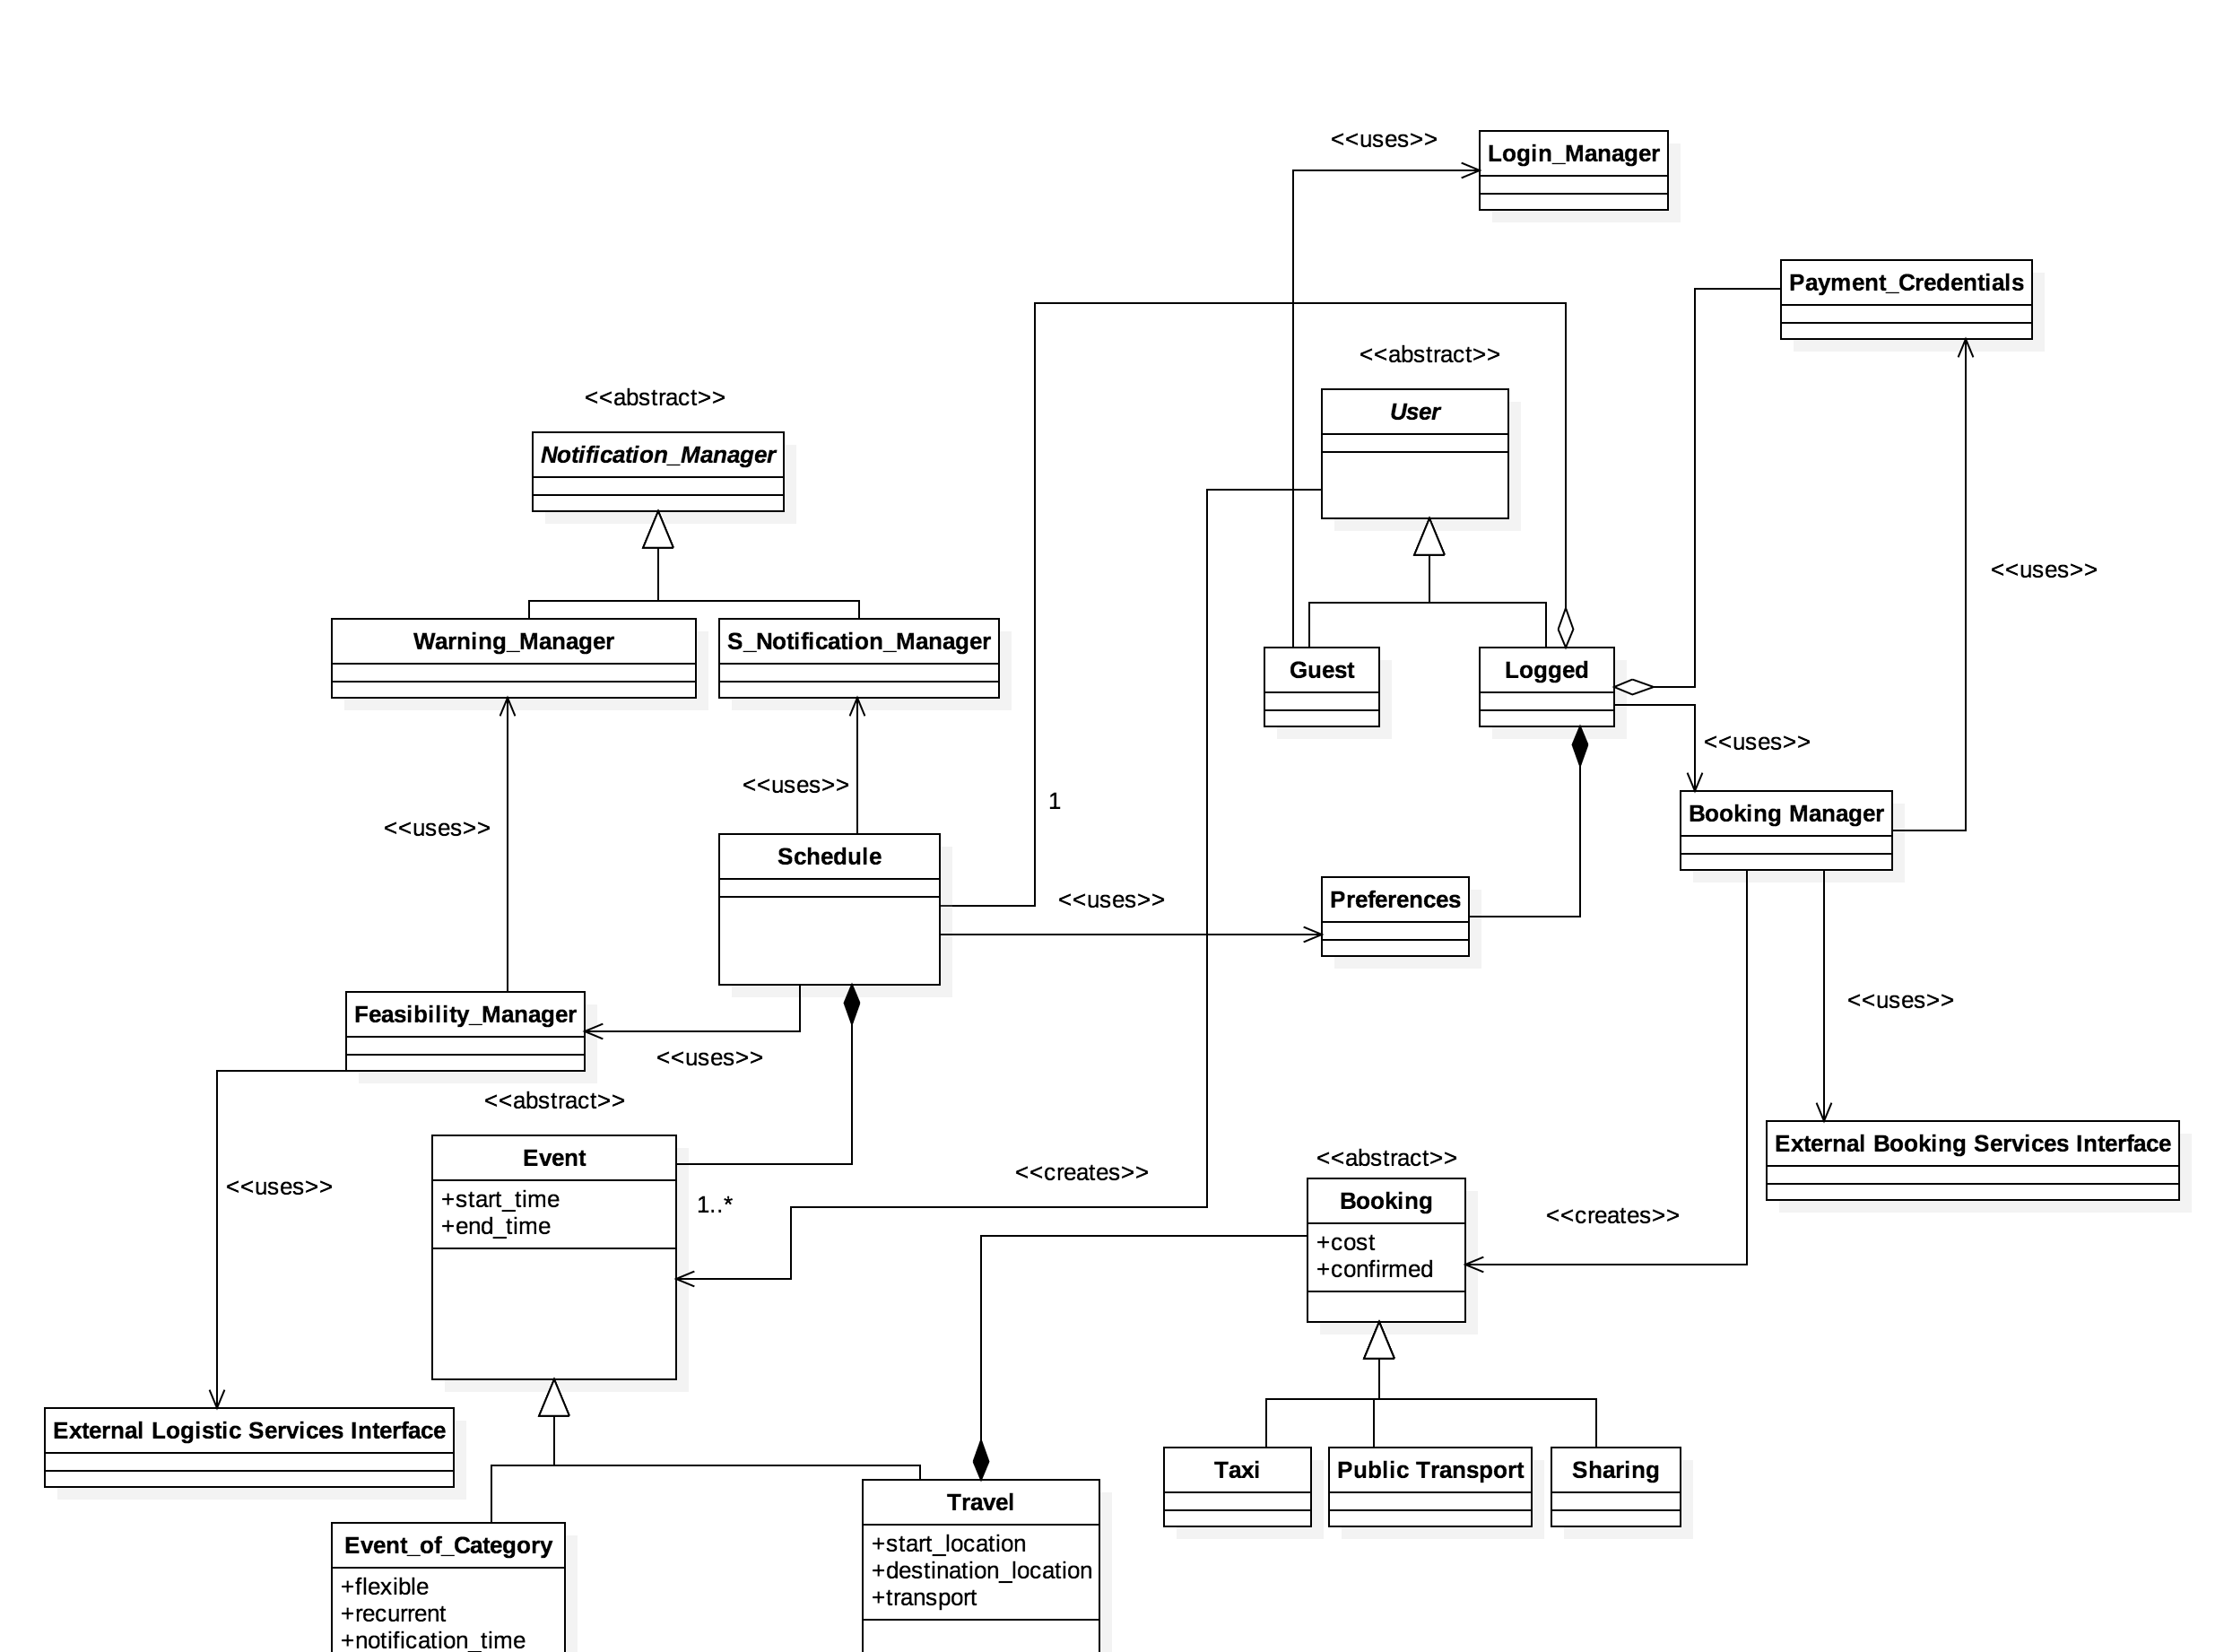
\includegraphics[width=1\textwidth]{classdiagram}
	\caption{\textit{Travlendar+} Class Diagram}
\end{figure}

\subsubsection{State Chart Diagrams}

\begin{figure}[H]
	\centering
	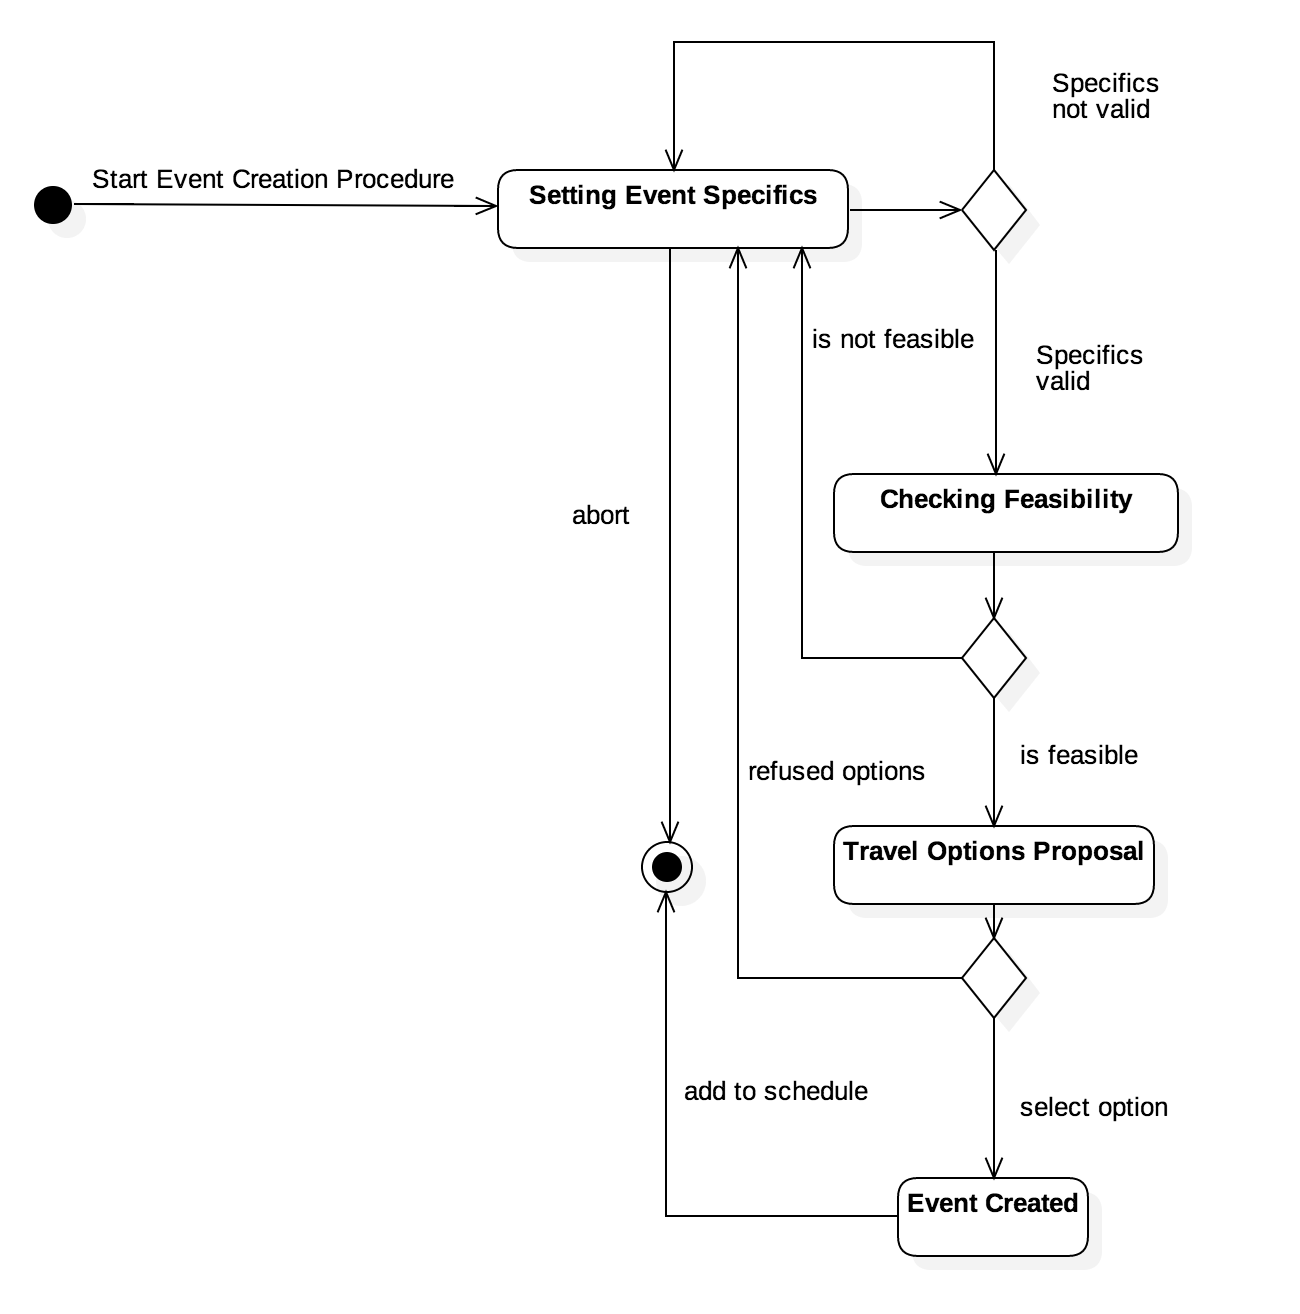
\includegraphics[width=1\textwidth]{eventadd}
	\caption{Add event state chart}
\end{figure}

\begin{figure}[H]
	\centering
	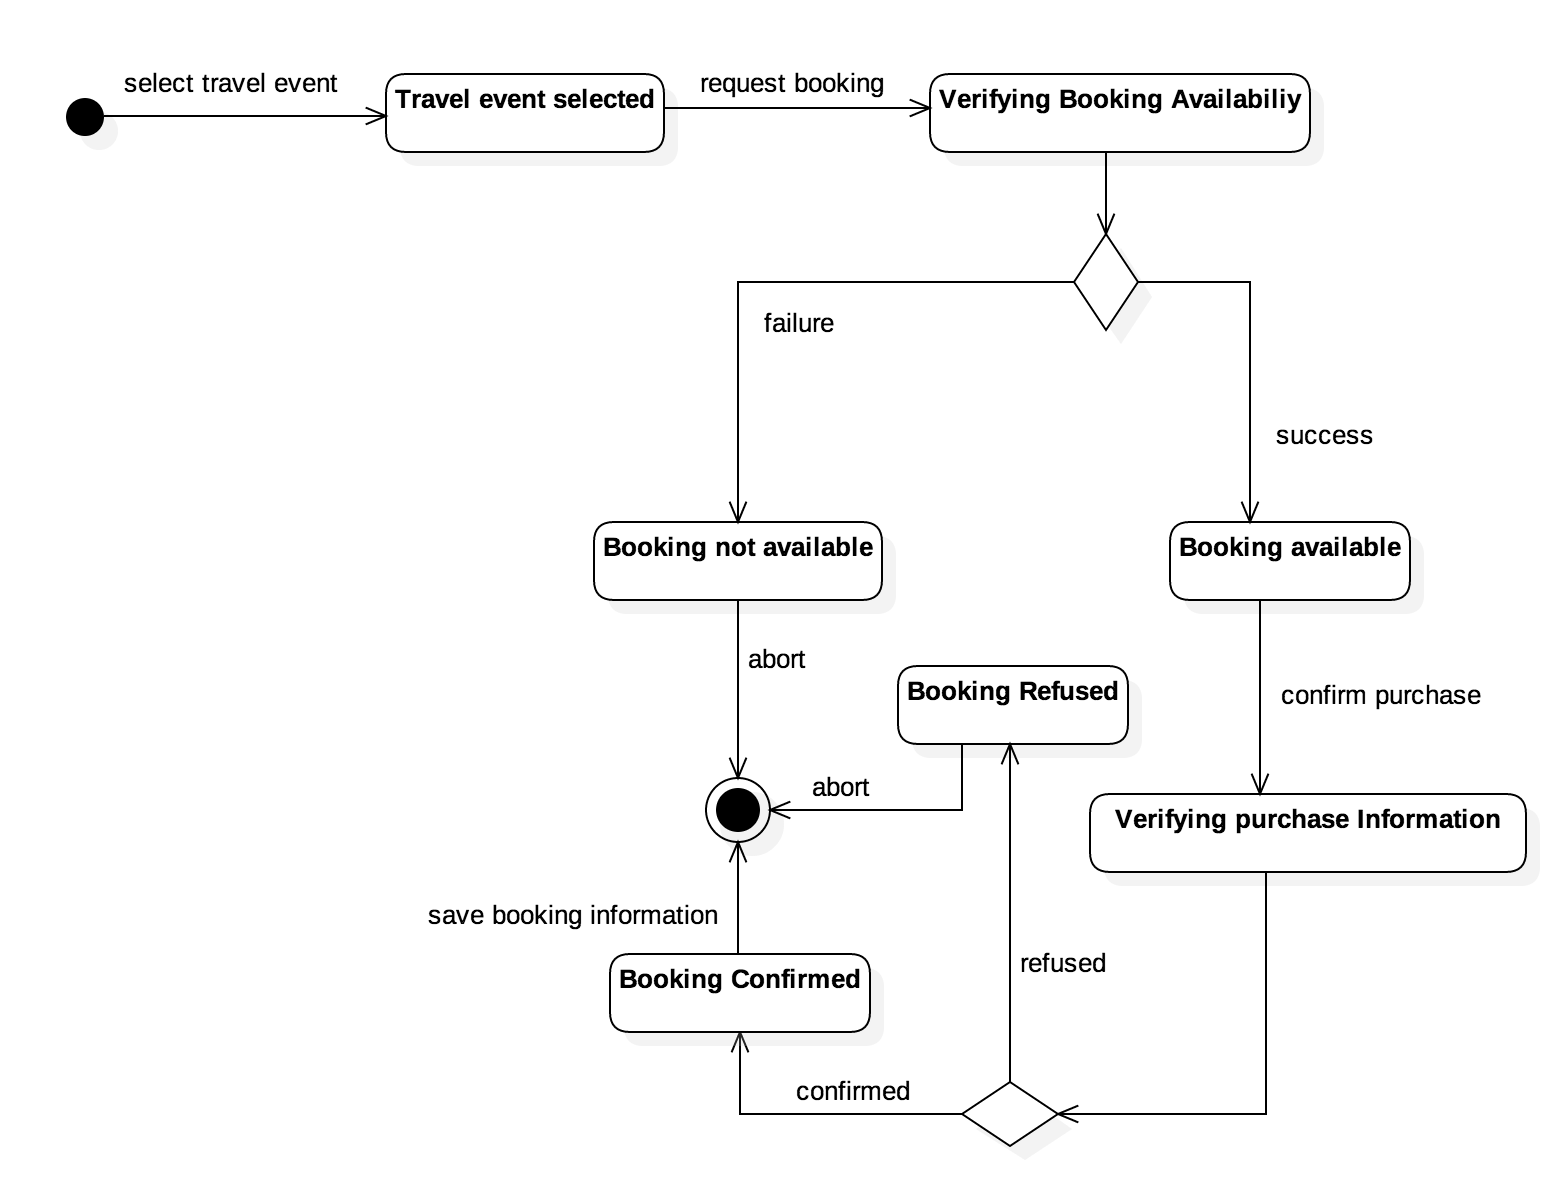
\includegraphics[width=1\textwidth]{booktravel}
	\caption{Booking travel state chart}
\end{figure}

\newpage
\subsubsection{Use Case Diagrams}

\begin{figure}[H]
	\centering
	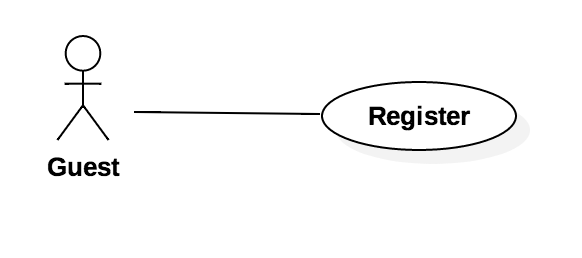
\includegraphics[width=0.5\textwidth]{actorguest}
	\caption{Guest use case}
\end{figure}

\begin{figure}[H]
	
	\centering
	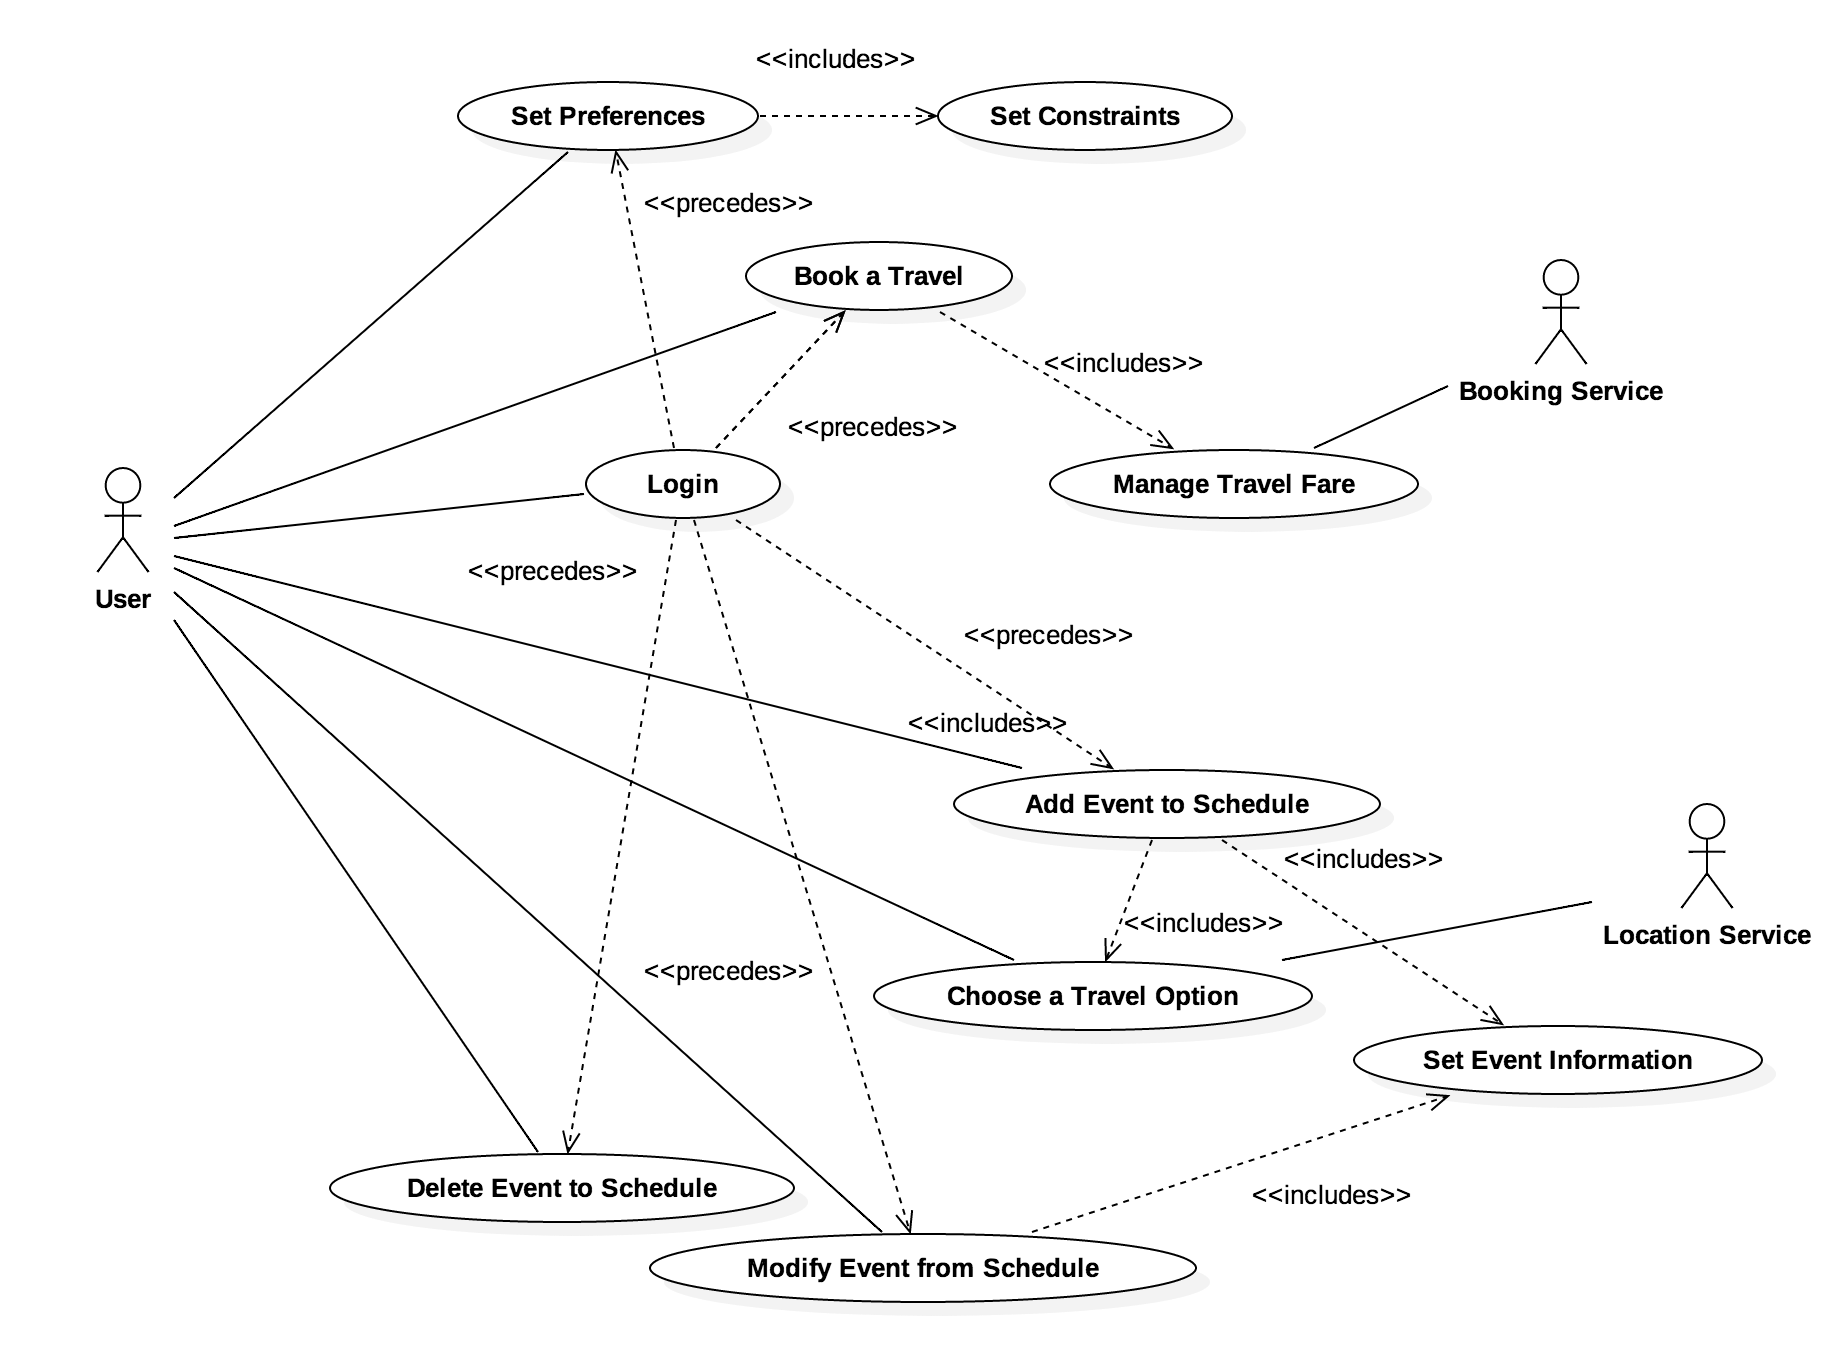
\includegraphics[width=1\textwidth]{actoruser}
	\caption{User use case}
\end{figure}

\newpage
\subsubsection{Use Case Templates}
\begin{center}
	\textbf{Register Account}
\end{center}

\begin{tabularx}{\linewidth}{| l | X |}
	\hline
	\textbf{ID} & UC1\\
	
	\hline
	\textbf{Description} & The \textbf{\textit{Guest}} wants to create an account for the application.\\
	
	\hline
	\textbf{Actors} & \textbf{\textit{Guest}}\\
	
	\hline
	\textbf{Preconditions} & The \textbf{\textit{Guest}} opened the application\\
	
	\hline
	\textbf{Flow of Events} & \parbox{0.7\textwidth}{\begin{enumerate}
			\item The \textbf{\textit{Guest}} selects the function \textit{Sign Up}.
			\item The \textbf{\textit{System}} returns a form to enter all the required data: username, email address and password which will be used for the future logins.
			\item The \textbf{\textit{Guest}} fills the form with all the required information.
			\item The \textbf{\textit{User Manager}} checks if all the informations are correct, generates a random activation URL and asks the \textbf{\textit{Mailing System}} to forward his/her URL to the email address of the \textbf{\textit{Guest}}.
			\item The \textbf{\textit{Guest}} receives the mail and click on the URL. The \textbf{\textit{User Manager}} stores the data provided by the \textbf{\textit{User}}.
	\end{enumerate}}\\
	
	\hline
	\textbf{Postconditions} & The \textbf{\textit{Guest}} is able to sign in.\\
	
	\hline
	\textbf{Exceptions} & \parbox{0.7\textwidth}{ \begin{enumerate}
			\item The \textbf{\textit{User Manager}} recognizes invalid information than shows an error message. The flow restarts from point 2.
		\end{enumerate}}\\
	
	\hline
	
\end{tabularx}
\newpage
\begin{center}
	\textbf{Log In}
\end{center}

\begin{tabularx}{\linewidth}{| l | X |}
	\hline
	\textbf{ID} & UC2\\
	
	\hline
	\textbf{Description} & The \textbf{\textit{User}} wants to log in to the application.\\
	
	\hline
	\textbf{Actors} & \textbf{\textit{User}}\\
	
	\hline
	\textbf{Preconditions} & The \textbf{\textit{User}} opened the application\\
	
	\hline
	\textbf{Flow of Events} & \parbox{0.7\textwidth}{\begin{enumerate}
			\item The \textbf{\textit{User}} inserts his/her credentials.
			\item The \textbf{\textit{User}} taps the \textit{Sign In} button.
			\item The \textbf{\textit{User Manager}} checks provided credentials.
	\end{enumerate}}\\
	
	\hline
	\textbf{Postconditions} & The \textbf{\textit{User}} is logged in.\\
	
	\hline
	\textbf{Exceptions} & \parbox{0.7\textwidth}{ \begin{enumerate}
			\item The \textbf{\textit{User Manager}} recognizes invalid credentials then shows an error message. The flow restarts from point 2.
	\end{enumerate}}\\
	
	\hline
	
\end{tabularx}

%\begin{center}
%	\textbf{Log out}
%\end{center}
%
%\begin{tabularx}{\linewidth}{| l | X |}
%	\hline
%	\textbf{ID} & UC3\\
%	
%	\hline
%	\textbf{Description} & The \textbf{\textit{User}} wants to log out of the \textbf{\textit{Travlendar+}} application.\\
%	
%	\hline
%	\textbf{Actors} & \textbf{\textit{User}}\\
%	
%	\hline
%	\textbf{Preconditions} & The \textbf{\textit{User}} is logged in to the application.\\
%	
%	\hline
%	\textbf{Flow of Events} & \parbox{0.7\textwidth}{\begin{enumerate}
%			\item The \textbf{\textit{User}} opens the menu.
%			\item The \textbf{\textit{User}} tap the \textit{Log Out} section.
%			\item The \textbf{\textit{Notification Manager}} displays a confirmation message.
%			\item The \textbf{\textit{User}} selects \textit{yes}.
%			\item The \textbf{\textit{System}} performs the \textbf{\textit{User's}} log out.
%	\end{enumerate}}\\
%	
%	\hline
%	\textbf{Postconditions} & The \textbf{\textit{User}} is logged out.\\
%	
%	\hline
%	\textbf{Exceptions} & \parbox{0.7\textwidth}{ \begin{enumerate}
%			\item The \textbf{\textit{User}} selects the \textit{No} option. The flow of events restarts from point 1.
%	\end{enumerate}}\\
%	
%	\hline
%	
%\end{tabularx}

\begin{center}
	\textbf{Set User Settings}
\end{center}

\begin{tabularx}{\linewidth}{| l | X |}
	\hline
	\textbf{ID} & UC4\\
	
	\hline
	\textbf{Description} & The \textbf{\textit{User}} wants to set User settings.\\
	
	\hline
	\textbf{Actors} & \textbf{\textit{User}}\\
	
	\hline
	\textbf{Preconditions} & The \textbf{\textit{User}} is logged in to the application.\\
	
	\hline
	\textbf{Flow of Events} & \parbox{0.7\textwidth}{\begin{enumerate}
			\item The \textbf{\textit{User}} opens the menu.
			\item The \textbf{\textit{User}} taps the \textit{User Settings} section.
			\item The \textbf{\textit{System}} displays the \textit{User Settings} view.
			\item The \textbf{\textit{User}} changes his/her personal informations and clicks the \textit{Confirm} button.
	\end{enumerate}}\\
	
	\hline
	\textbf{Postconditions} & The \textbf{\textit{User}} changed his personal informations.\\
	
	\hline
	\textbf{Exceptions} & \parbox{0.7\textwidth}{\begin{enumerate}
			\item The \textbf{\textit{User Manager}} recognizes invalid credentials then shows an error message. The flow restarts from point 3.
		\end{enumerate}}\\
	
	\hline
	
\end{tabularx}

\begin{center}
	\textbf{Set Travel Preferences}
\end{center}

\begin{tabularx}{\linewidth}{| l | X |}
	\hline
	\textbf{ID} & UC5\\
	
	\hline
	\textbf{Description} & The \textbf{\textit{User}} wants to set travel preferences.\\
	
	\hline
	\textbf{Actors} & \textbf{\textit{User}}\\
	
	\hline
	\textbf{Preconditions} & The \textbf{\textit{User}} is logged in to the application.\\
	
	\hline
	\textbf{Flow of Events} & \parbox{0.7\textwidth}{\begin{enumerate}
			\item The \textbf{\textit{User}} opens the menu.
			\item The \textbf{\textit{User}} taps the \textit{Travel Preferences} section.
			\item The \textbf{\textit{System}} displays the \textit{Travel Preferences} view.
			\item The \textbf{\textit{User}} selects/deselects each travel mean and set specific constraint for the selected ones.
			\item The \textbf{\textit{User}} clicks on the \textit{Confirm} button.
	\end{enumerate}}\\
	
	\hline
	\textbf{Postconditions} & The \textbf{\textit{User}} changed his/her travel preferences. \\
	
	\hline
	\textbf{Exceptions} & \parbox{0.7\textwidth}{}\\
	
	\hline
	
\end{tabularx}

\begin{center}
	\textbf{Add normal and flexible event}
\end{center}

\begin{tabularx}{\linewidth}{| l | X|}
	\hline
	\textbf{ID} & UC6\\
	
	\hline
	\textbf{Description} & The \textbf{\textit{User}} wants to add a normal or flexible event to the schedule.\\
	
	\hline
	\textbf{Actors} & \textbf{\textit{User}}\\
	
	\hline
	\textbf{Preconditions} & The \textbf{\textit{User}} is logged in to the application and is in the \textit{Schedule} or \textit{Calendar} section.\\
	
	\hline
	\textbf{Flow of Events} & \parbox{0.7\textwidth}{\begin{enumerate}
			\item The \textbf{\textit{User}} clicks the \textit{Add} button.
			\item The \textbf{\textit{System}} returns a form to enter all the required data: name, position of the event, previous position (from where the appointment will be reached), start and end time.
			\item The \textbf{\textit{User}} fills all the required fields.
			\item The \textbf{\textit{User}} clicks the \textit{Confirm} button.
			\item The \textbf{\textit{Feasibility Manager}} checks the schedulability of the event.
			\item The \textbf{\textit{System}} calculates the best travel means options and proposes them to the \textbf{\textit{User}}.
			\item The \textbf{\textit{User}} selects a travel mean.
	\end{enumerate}}\\
	\hline
	
	\textbf{Postconditions} & The \textbf{\textit{User}} added the event to his/her schedule. \\
	
	\hline
	\textbf{Exceptions} & \parbox{0.7\textwidth}{ \begin{enumerate}
		\item The \textbf{\textit{Feasibility Manager}} detects a conflict in the schedule. The \textbf{\textit{Warning Manager}} displays a warning message. The flow restarts from point 2.
		\item The \textbf{\textit{User}} did not correctly compile the form before clicking \textit{Confirm}. The flow restarts from point 2.
	\end{enumerate}}\\
	
	\hline
	
\end{tabularx}

\begin{center}
	\textbf{Add repetitive event}
\end{center}

\begin{tabularx}{\linewidth}{| l | X|}
	\hline
	\textbf{ID} & UC7\\
	
	\hline
	\textbf{Description} & The \textbf{\textit{User}} wants to add a repetitive event to the schedule.\\
	
	\hline
	\textbf{Actors} & \textbf{\textit{User}}\\
	
	\hline
	\textbf{Preconditions} & The \textbf{\textit{User}} is logged in to the application and is in the \textit{Schedule} or \textit{Calendar} section.\\
	
	\hline
	\textbf{Flow of Events} & \parbox{0.68\textwidth}{\begin{enumerate}
			\item The \textbf{\textit{User}} clicks the \textit{Add} button.
			\item The \textbf{\textit{System}} returns a form to enter all the required data.
			\item The \textbf{\textit{User}} selects the \textit{Repetitive} option.
			\item The \textbf{\textit{System}} shows the form relative to the repetitive event.
			\item The \textbf{\textit{User}} fills the form and clicks the \textit{Confirm} button.
			\item The \textbf{\textit{Feasibility Manager}} checks the schedulability for all the repetitions of the event.
	\end{enumerate}}\\
	
	\hline
	\textbf{Alternative Flow} & \parbox{0.68\textwidth}{ \begin{enumerate}
			\setcounter{enumi}{6}
			\item The \textbf{\textit{Feasibility Manager}} detects a conflict in the schedule. 
			\item The \textit{\textbf{System}} asks the \textbf{\textit{User}} whether schedule the event only in the days without conflict. 
			\item The \textbf{\textit{User}} chooses to proceed with the creation.
	\end{enumerate}}\\

	\hline
	
	\textbf{Postconditions} & The \textbf{\textit{User}} added the repetitive event to his/her schedule. \\
	
	\hline
	\textbf{Exceptions} & \parbox{0.68\textwidth}{ \begin{enumerate}
			\item The \textbf{\textit{User}} did not correctly compile the form before clicking \textit{Confirm}. The flow restarts from point 2.
			\item The \textbf{\textit{User}} chooses to stop the creation of the event. The flow restarts from point 4.
	\end{enumerate}}\\
	
	\hline
	
\end{tabularx}

\begin{center}
	\textbf{Delete event}
\end{center}

\begin{tabularx}{\linewidth}{| l | X |}
	\hline
	\textbf{ID} & UC8\\
	
	\hline
	\textbf{Description} & The \textbf{\textit{User}} wants to delete an event from a schedule.\\
	
	\hline
	\textbf{Actors} & \textbf{\textit{User}}\\
	
	\hline
	\textbf{Preconditions} & The \textbf{\textit{User}} is in the \textit{Home} or in the \textit{Schedule} section of a particular day.\\
	
	\hline
	\textbf{Flow of Events} & \parbox{0.7\textwidth}{\begin{enumerate}
			\item The \textbf{\textit{User}} clicks the \textit{Delete} button on a particular scheduled event.
			\item The \textbf{\textit{Warning Manager}} shows a warning message and ask the \textbf{\textit{User}} to confirm his/her choice.
			\item The \textbf{\textit{User}} clicks the \textit{Yes} button.
	\end{enumerate}}\\
	
	\hline
	\textbf{Postconditions} & The \textbf{\textit{User}} deleted an event from the schedule. \\
	
	\hline
	\textbf{Exceptions} & \parbox{0.7\textwidth}{ \begin{enumerate}
			\item The \textbf{\textit{User}} clicked the \textit{No} button in the warning message.
	\end{enumerate}}\\
	
	\hline
	
\end{tabularx}

\begin{center}
	\textbf{Edit event}
\end{center}

\begin{tabularx}{\linewidth}{| l | X |}
	\hline
	\textbf{ID} & UC9\\
	
	\hline
	\textbf{Description} & The \textbf{\textit{User}} wants to modify an event from a schedule.\\
	
	\hline
	\textbf{Actors} & \textbf{\textit{User}}\\
	
	\hline
	\textbf{Preconditions} & The \textbf{\textit{User}} is in the \textit{Home} or in the \textit{Schedule} section of a particular day.\\
	
	\hline
	\textbf{Flow of Events} & \parbox{0.7\textwidth}{\begin{enumerate}
			\item The \textbf{\textit{User}} clicks the \textit{Edit} button on a particular scheduled event.
			\item The \textit{\textbf{System}} shows the edit page.
			\item The \textit{\textbf{User}} can modify the event informations.
			\item The \textit{\textbf{User}} clicks the \textit{Confirm} button.
			\item The \textbf{\textit{Feasibility Manager}} checks the schedulability of the event.
			\item The \textbf{\textit{System}} calculates the best travel mean options and propose them to the \textbf{\textit{User}}.
			\item The \textbf{\textit{User}} selects a travel mean.
	\end{enumerate}}\\
	
	\hline
	\textbf{Postconditions} & The \textbf{\textit{User}} edited the event. \\
	
	\hline
	\textbf{Exceptions} & \parbox{0.7\textwidth}{ \begin{enumerate}
			\item The \textbf{\textit{Feasibility Manager}} detects a conflict in the schedule. The \textbf{\textit{Warning Manager}} displays a warning message. The flow restarts from point 2.
	\end{enumerate}}\\
	
	\hline
	
\end{tabularx}


\begin{center}
	\textbf{Book travel}
\end{center}

\begin{tabularx}{\linewidth}{| l | X |}
	\hline
	\textbf{ID} & UC10\\
	
	\hline
	\textbf{Description} & The \textbf{\textit{User}} wants to buy a ticket or book a ride for a travel.\\
	
	\hline
	\textbf{Actors} & \textbf{\textit{User}}\\
	
	\hline
	\textbf{Preconditions} & The \textbf{\textit{User}} is in the \textit{Home} or in the \textit{Schedule} section of a particular day.\\
	
	\hline
	\textbf{Flow of Events} & \parbox{0.7\textwidth}{\begin{enumerate}
			\item The \textbf{\textit{User}} clicks the \textit{Buy} button on a specific scheduled event.
			\item The \textbf{\textit{System}} checks the availability of the requested service and redirect the \textbf{\textit{User}} to the specific third party service which will manage the \textit{User's} request.
			\item The \textbf{\textit{User}} provides his/her credentials to the third party service.
	\end{enumerate}}\\
	
	\hline
	\textbf{Postconditions} & The \textbf{\textit{User}} bought a ticket or booked a ride for a travel to reach the associated event. \\
	
	\hline
	\textbf{Exceptions} & \parbox{0.7\textwidth}{ \begin{enumerate}
			\item The booking service in point 2 is not available. The \textit{\textbf{Warning Manager}} shows a warning message and the booking process stops.
			\item The credential provided by the \textbf{\textit{User}} in point 3 are not correct. The \textbf{\textit{Warning Manager}} shows a warning message and the flow restart from point 3.
	\end{enumerate}}\\
	\hline
\end{tabularx}

\subsubsection{Sequence Diagrams}

\begin{figure}[H]
	\centering
	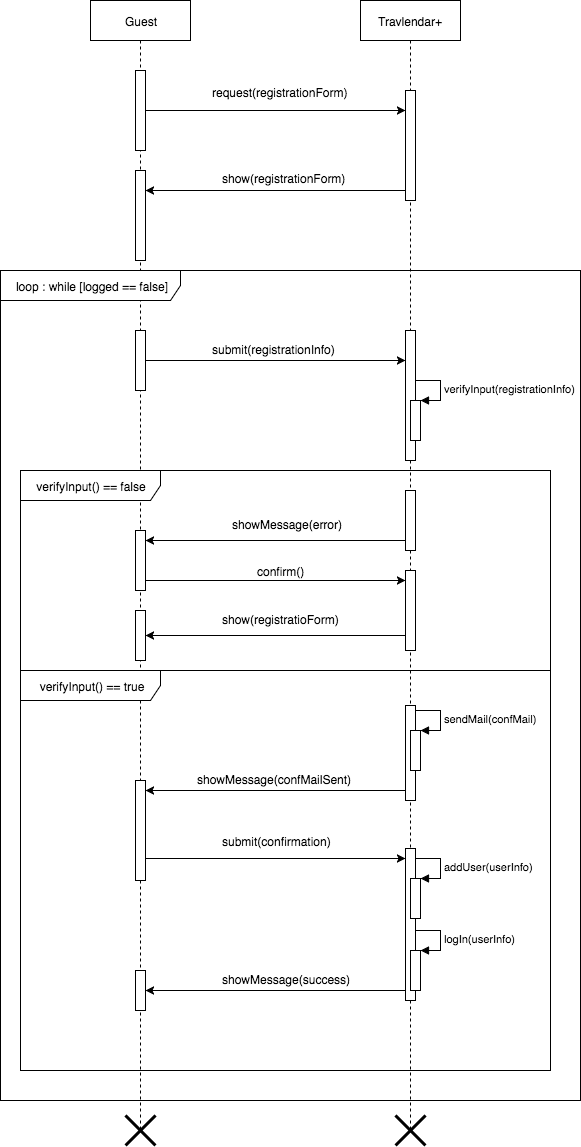
\includegraphics[width=0.69\textwidth]{SequenceDiagramSignup}
	\caption{Sign Up sequence diagram}
\end{figure}

\begin{figure}[H]
	\centering
	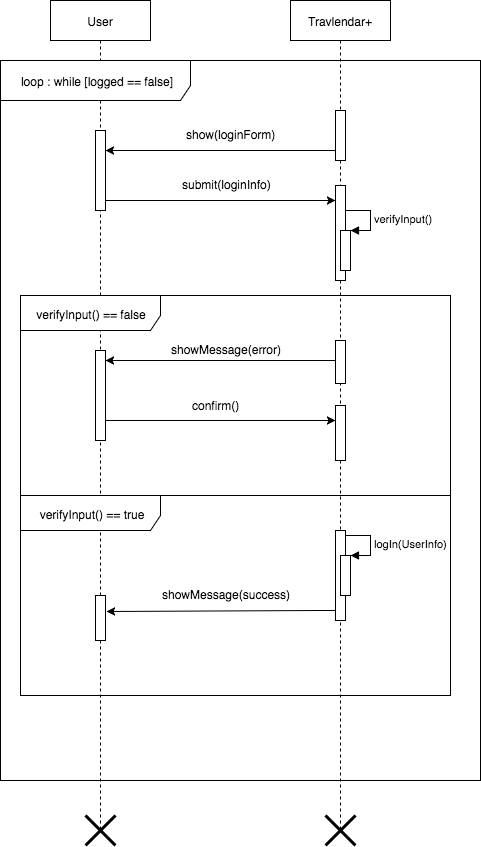
\includegraphics[width=0.8\textwidth]{SequenceDiagramLogin}
	\caption{Log In sequence diagram}
\end{figure}

\begin{figure}[H]
	\centering
	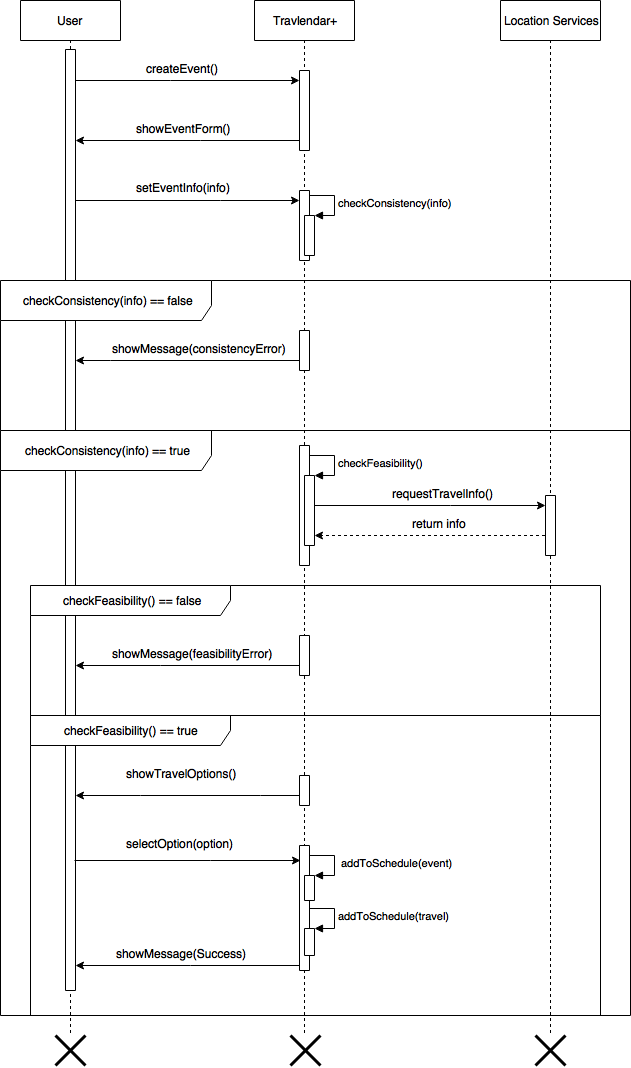
\includegraphics[width=0.8\textwidth]{SequenceDiagramEventCreation}
	\caption{Normal and Flexible event creation sequence diagram}
\end{figure}

\begin{figure}[H]
	\centering
	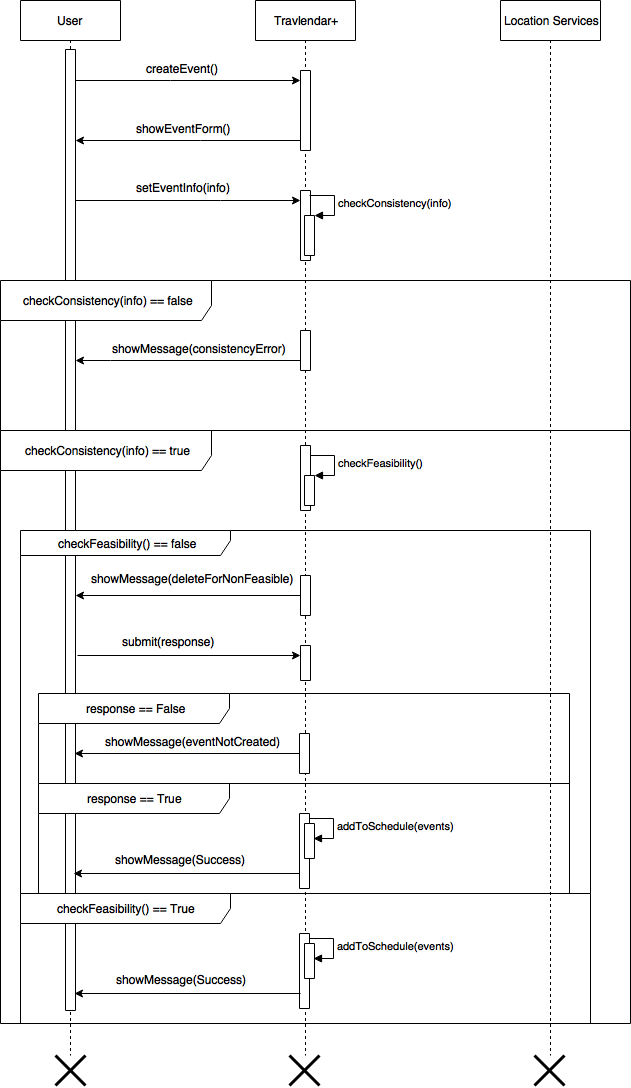
\includegraphics[width=0.8\textwidth]{SequenceDiagramRepetitiveEventCreation}
	\caption{Recurrent event creation sequence diagram}
\end{figure}


\begin{figure}[H]
	\centering
	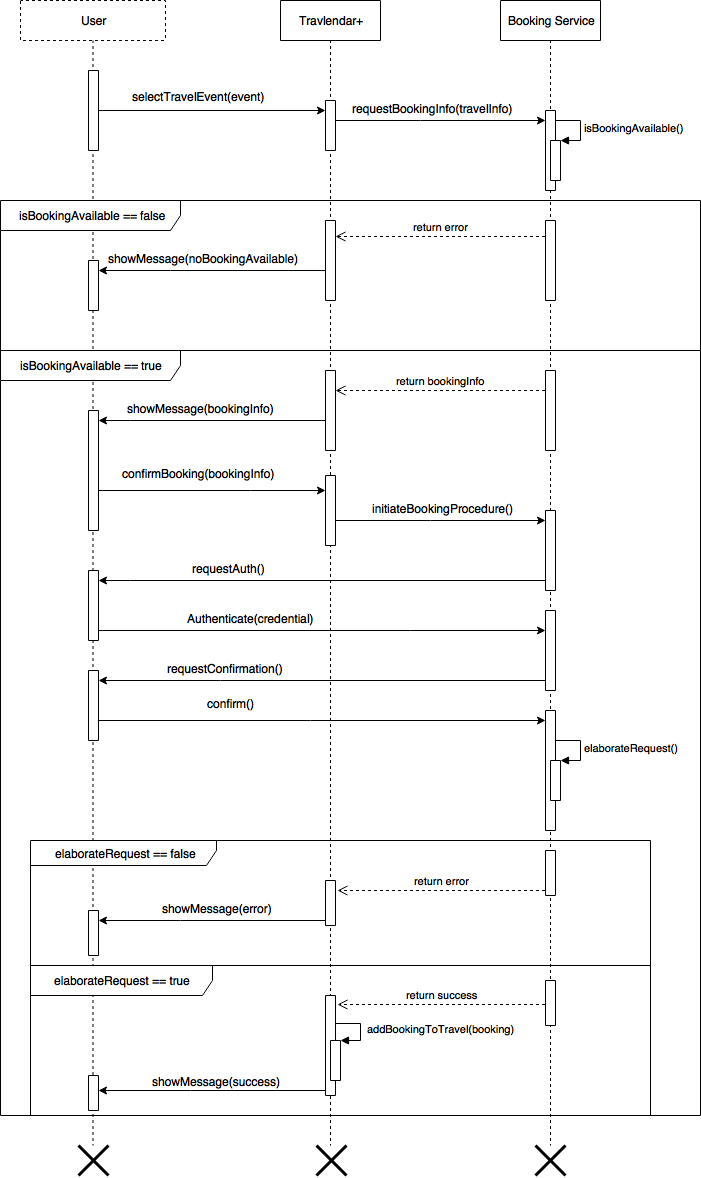
\includegraphics[width=0.8\textwidth]{SequenceDiagramTravelBooking}
	\caption{Travel booking sequence diagram}
\end{figure}

\newpage
\subsection{Product Functions}
In this section the most important features of the application are explained.

\begin{itemize}
	\item \textbf{Manage meetings}\\
	The System allows the User to add, edit and delete events in the schedule for a particular day. During the creation of the event, the User must specify the name of the event, the time and date of start and end of the event, the location of the event and the location from which it will be reached. Furthermore, the User will be able to add additional information about the event such as a briefly description and a category.\\
	For each event, the User is also provided with a list of possible travel means: the System will compute the best travel mean options accordingly with the information provided and the Users' travel preferences. The User will then be able to select one of the mean of transportation proposed.\\
	The User is also able to modify informations about a specific event or to delete it.\\
	The System guarantees the feasibility of the schedule for each day. To do this, it allows the User to add or edit only events in the schedule that are not in conflict with the ones already present.\\
	Finally, the User can choose to be notified a certain time before the event.
	
	
	\item \textbf{Set travel preferences}\\
	The User is able to customize his/her travel preferences globally activating or deactivating travel means that are:
	\begin{itemize}
		\item Personal motor vehicle
		\item Public transport
		\item Personal bicycle
		\item Taxi services
		\item Car sharing services
		\item Bike sharing services
		\item On foot
	\end{itemize} 
	Furthermore, for each travel mean a set of editable constraints is provided. The System gives also the possibility to activate an \textit{Eco Mode} option: in this case, the best travel solution will be computed in order to minimize carbon footprint.
	
	\item \textbf{Create flexible and repetitive events}\\
	The User is allowed to create flexible and repetitive events. Flexible events are particular type of events in which the User, besides the information about event date and location, must specify a window of time where the event can occur and a duration. In order to preserve the feasibility of the schedule, the System can arbitrarily move the event inside the window's bounds.\\
	On the other hand, repetitive events are particular type of events that are repeated with a frequency specified by the User. For these type of events, the User will be able to provide informations about start and end time and location, but will not be able to select a global travel means. For each occurrence of the event, the User will be allowed to request travel options and choose a travel mean.
	
	\item \textbf{Transport booking}\\
	The System provides a way to book some of the travel means proposed during the schedule phase relying on third party services. The User will be automatically redirected to the app or to the site of the service supplier to complete the purchase.
	However, the System provides only an interface for these services: the User might be requested to sign up/log in and to provide payment information in order to buy a ticket or book a ride. All the operations which occur in this phase are totally performed out of the application.
\end{itemize}

\subsection{User Characteristics}
\textit{Travlendar+} is suitable for all kind of Users, with no age limit.
We give for granted that both Users have access to Internet and are able to install and use the mobile application.\\
The characters are:
\begin{itemize}
	\item \textit{Guest:} a person who downloads and opens the app but still has to sign up. He/she cannot use any of the functions provided by \textit{Travlendar+}.
	\item \textit{User:} a registered User who has to log-in in order to access any feature of the application. He/she can retrieve his/her personal data from any device with the app installed just providing credentials.
	\item \textit{Logged-in User:} a User who logged in to the application and can manage his personal schedule, edit personal information and preferences. In order to book travels, he/she might need to be registered on third-party services.
\end{itemize}

\subsection{Constraints, Dependencies, Assumptions}
\textbf{Constraints}
\begin{itemize}
	\item Users are located in Milan.
	\item Users must have a smartphone equipped with an OS compatible with the application.  
	\item Users must have Internet connection.
	\item The System must ask Users for the permission to acquire, store and process personal data. Therefore, the System must offer the possibility to the Users to delete their personal account and the associated data.
\end{itemize}

\noindent \textbf{Dependencies}
\begin{itemize}
	\item The System will rely on external APIs to retrieve informations about travel means and associated ETA. 
	\item Travel booking options are provided by external third party services.
	\item The System needs a DBMS in order to store and retrieve Users' data.
\end{itemize}

\noindent \textbf{Assumptions}
\begin{itemize}
	\item \textbf{[D.1]} The given email is assumed to be correct.
	\item \textbf{[D.2]} The sent email is assumed to be correctly received.
	\item \textbf{[D.3]} The events informations provided by the user are correct.
	\item\textbf{[D.4]} Event time constraint are respected by the User.
	\item \textbf{[D.5]} The informations about the event are correct.
	\item \textbf{[D.6]} The informations about available mobility options and related travel time are correct.
	\item \textbf{[D.7]} If selected, the private means of transport are available without any delay.
	\item \textbf{[D.8]} The start location of the travel is known and correct.
	\item \textbf{[D.9]} All selected travel means specified in the preferences are potentially available to the User.
	\item \textbf{[D.10]} A minimum walking distance is assumed in order to reach every mean of transport. Such distance will not be taken into account unless significant with respect to the travel time, meaning unless it influences the ETA by more than a minute.
	\item \textbf{[D.11]} The User is registered to the service which offers the booking option.
	\item \textbf{[D.12]} The System internal clock time used to provide notifications is correct.
\end{itemize}

\newpage
\section{Specific Requirements}

\subsection{External Interface Requirements}
The \textit{Travlendar+} application is a mobile based application.\\
In the following section, a more detailed description of the application is given, in terms of hardware, software and communication interfaces.\\
Are also given some basic prototypes of the User interface through mockups.
\subsubsection{User Interfaces}
Aiming at being as simple and intuitive as possible, the application has a UI which follows the principles of flat design.

\begin{itemize}
	\item \textbf{Logo}
	The logo of \textit{Travlendar+}, which will also be the logo icon for the app on smartphones, is minimal but elaborate at the same time.
	Multiple rounded rectangle and squares are combined in a way that makes possible to distinguish both the letter 't' and the symbol '+'. This logo will also be shown during the application opening phase. \\
	
	\begin{figure}[H]
		\centering
		
\includegraphics[width=0.17\textwidth]{logo_icon.png}
		\caption{Icon}
	\end{figure}

	\begin{figure}[H]
		\centering
		
\includegraphics[width=0.47\textwidth]{logo_inline.png}
		\caption{Logo}
	\end{figure}
	
	\newpage
	\item \textbf{Sign In/Sign up}\\
	This form is the first thing the User sees after opening the app. It allows the User to log in, signup or recover the password if lost. The registration module requires three mandatory fields..

	\begin{figure}[H]
		\centering
		\begin{subfigure}{0.25\textwidth}
			\centering
			
\includegraphics[width=\textwidth]{intro.png}
		\end{subfigure}
		~
		\begin{subfigure}{0.25\textwidth}
			\centering
			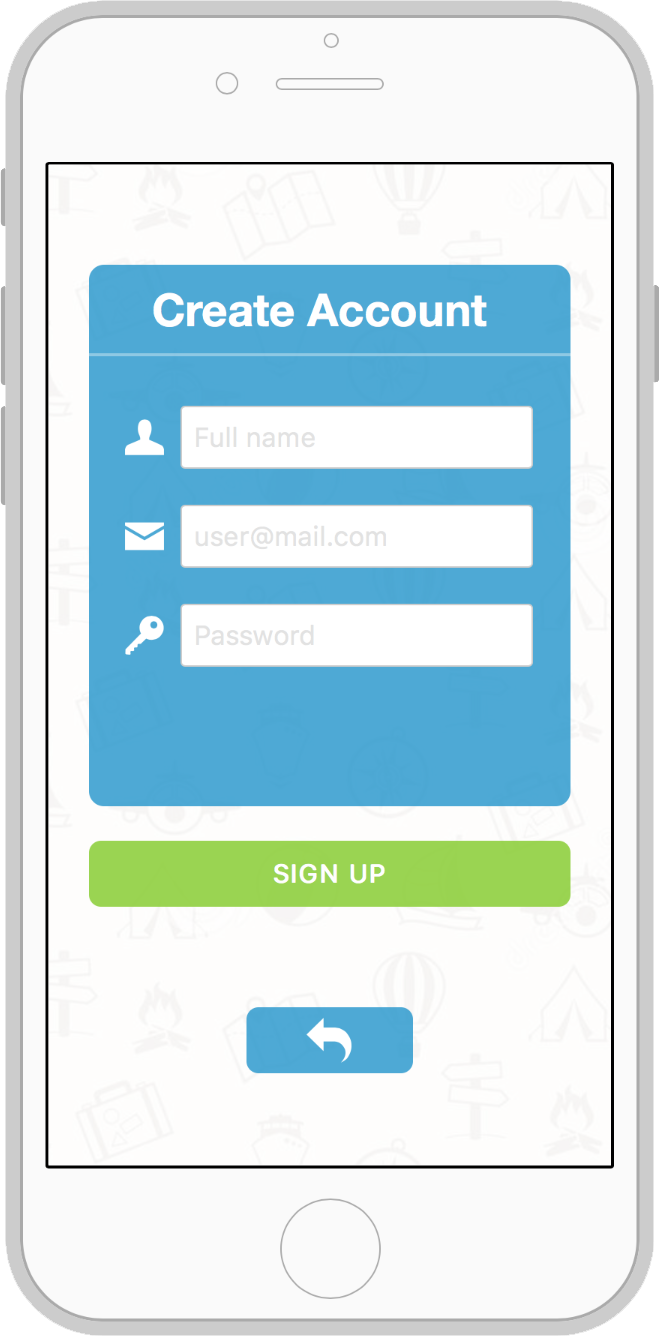
\includegraphics[width=\textwidth]{signup.png}
		\end{subfigure}
			~
	\begin{subfigure}{0.25\textwidth}
		\centering
		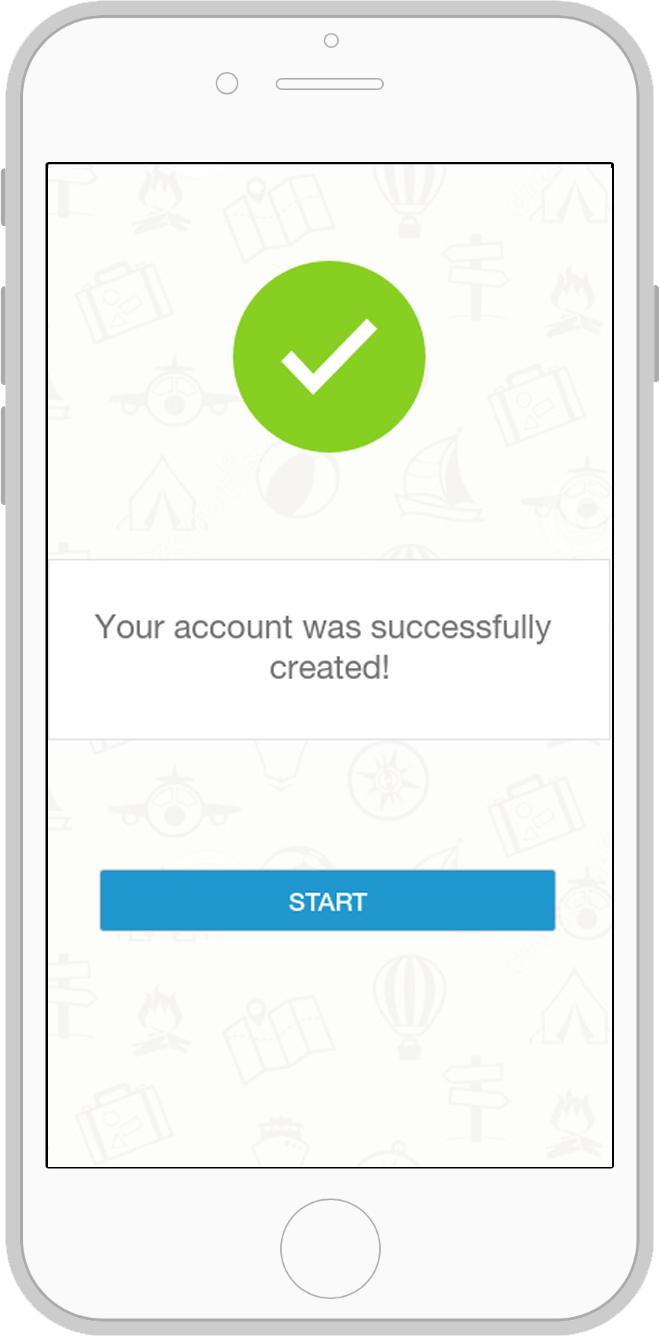
\includegraphics[width=\textwidth]{confirmation.png}
	\end{subfigure}
	\caption{Sign in and sign up procedures}
	\end{figure}

	\item \textbf{Home page}\\
	Contains all the events of the current day, which could be expanded and edited, and a button to add a new event for the current day.
	 %each event in order to see all the information about the transportation means, the trip route and all the preferences. Moreover the User is allowed to add a new event during the day or edit one of the already existent.\\
	%The User is able to access to all the other pages.
	\begin{figure}[H]
		\centering
		\begin{subfigure}{0.25\textwidth}
			\centering
			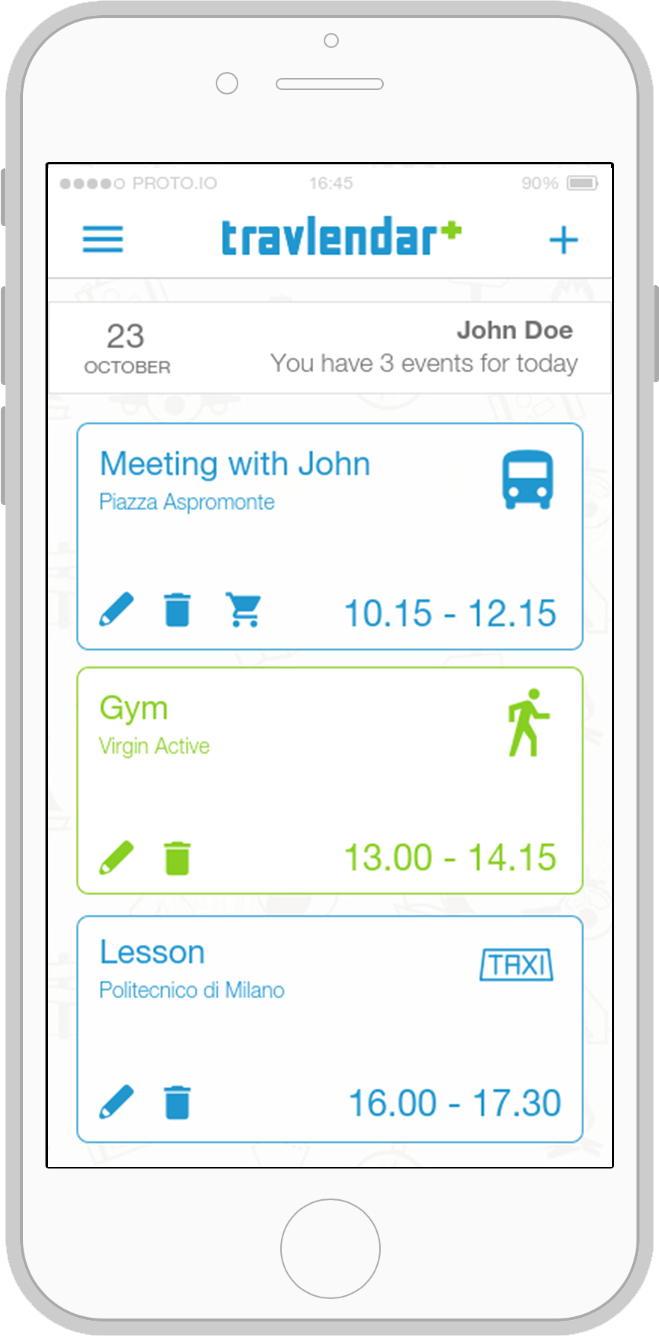
\includegraphics[width=\textwidth]{home_schedule.png}
		\end{subfigure}
	\caption{Daily schedule}
	\end{figure}

	\item \textbf{User settings}\\
	Used to view and edit the profile picture, personal email address, username and password.
	\begin{figure}[H]
	\centering
		\begin{subfigure}{0.25\textwidth}
		\centering
		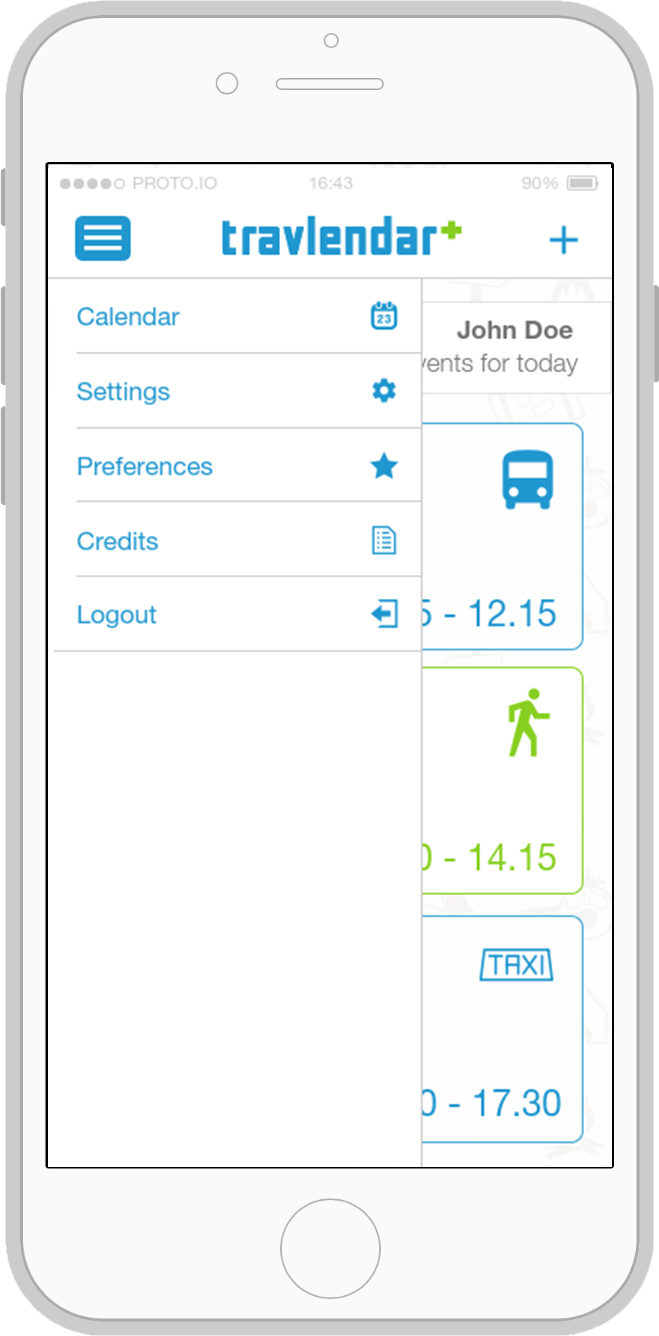
\includegraphics[width=\textwidth]{menu.png}
		\end{subfigure}
		~
		\begin{subfigure}{0.25\textwidth}
			\centering
			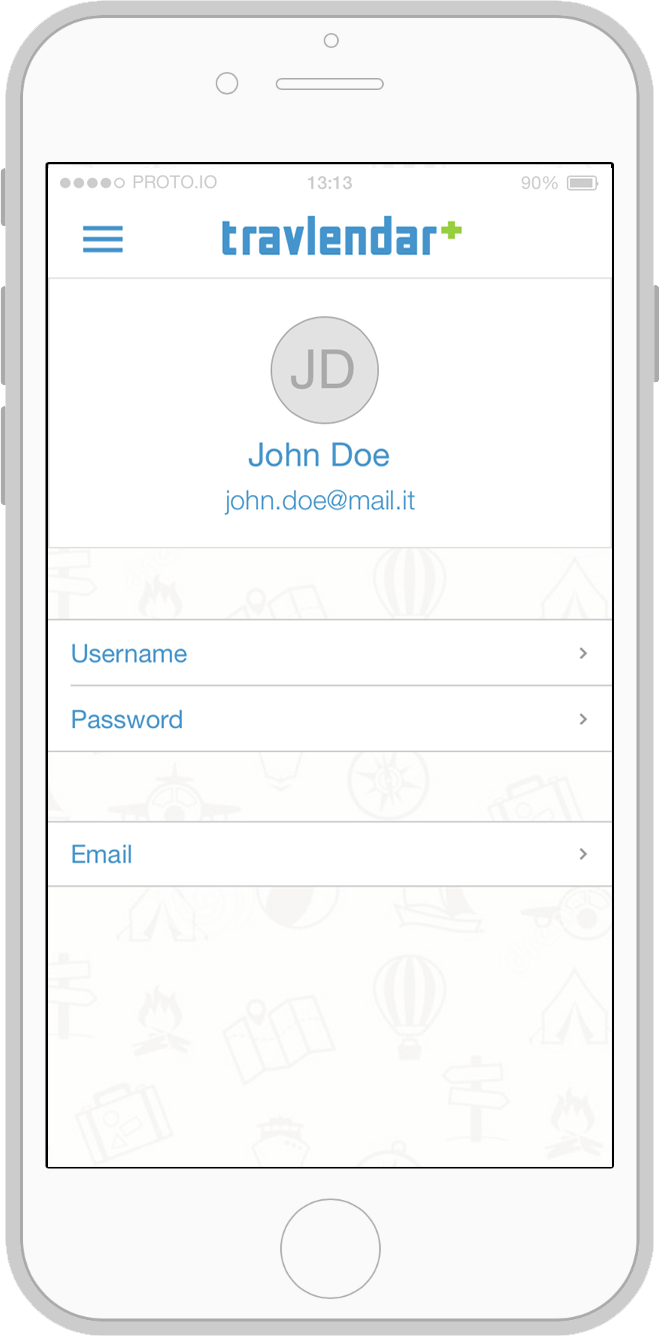
\includegraphics[width=\textwidth]{user_settings.png}
		\end{subfigure}

	\caption{Menu and User settings}
	\end{figure}

	\item \textbf{User preferences}\\
	In this page the User is able to activate or deactivate the available travel means and to set specific constraints for each of them.
	\begin{figure}[H]
		\centering
		\begin{subfigure}{0.25\textwidth}
			\centering
			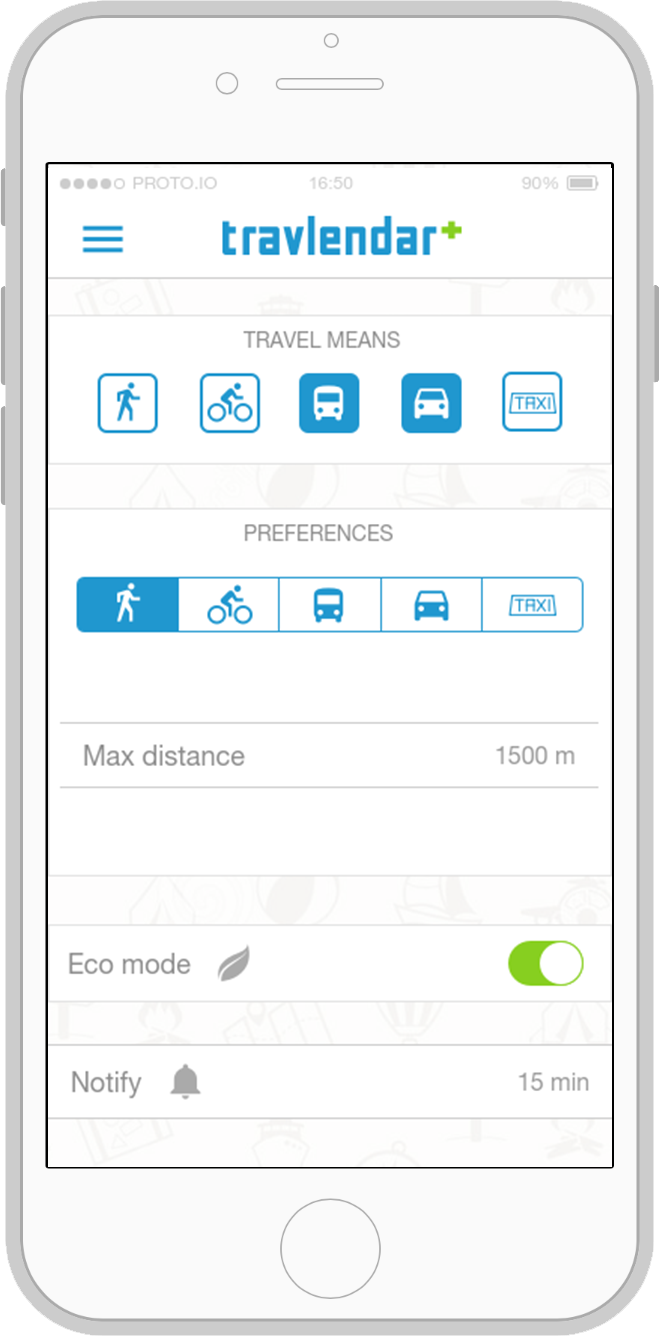
\includegraphics[width=\textwidth]{user_preferences.png}
		\end{subfigure}
		\caption{User preferences view}
	\end{figure}
	
	\item \textbf{Calendar page}\\
	Displays the  User calendar with a bullet for each day with at least one event scheduled. 
	\begin{figure}[H]
		\centering
		\begin{subfigure}{0.25\textwidth}
			\centering
			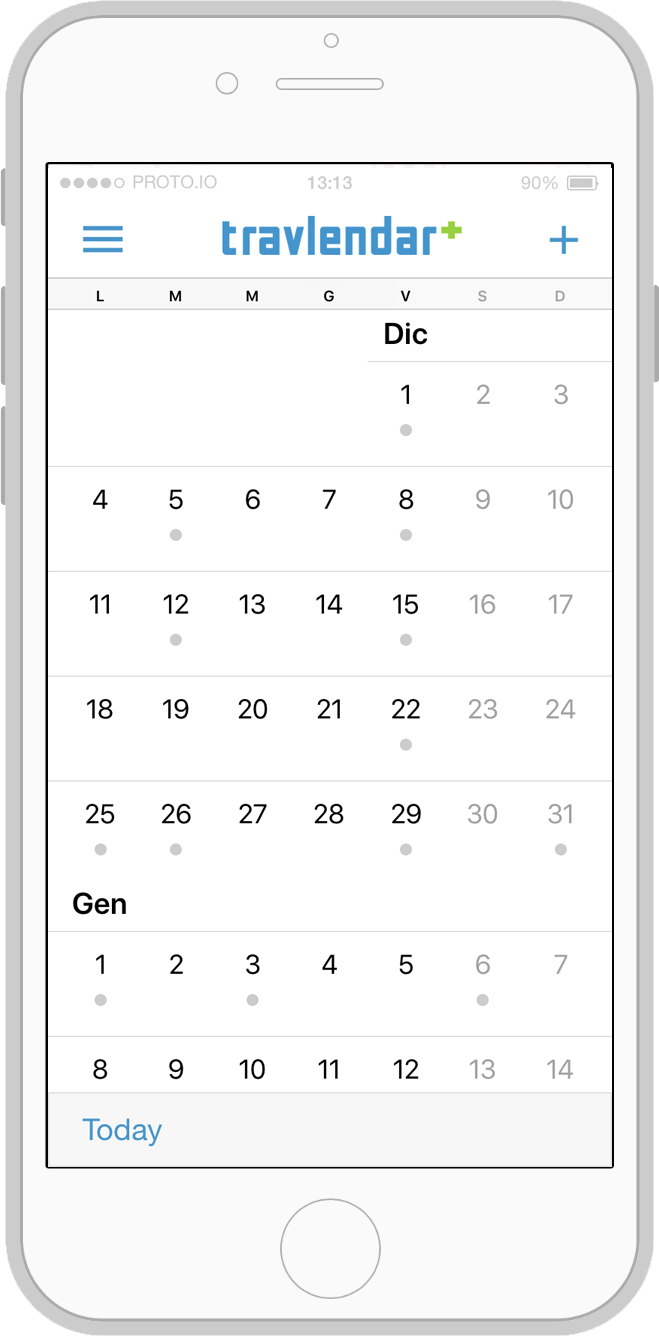
\includegraphics[width=\textwidth]{calendar.png}
		\end{subfigure}
		\caption{Calendar view}
	\end{figure}
		

	\item \textbf{New/Edit event}\\
	Opened when an User wants to add a new event to the calendar or to edit an existent one. If fields are consistent and there is no conflict in the schedule a list of possible travel options is shown.
	\begin{figure}[H]
		\centering
		\begin{subfigure}{0.25\textwidth}
			\centering
			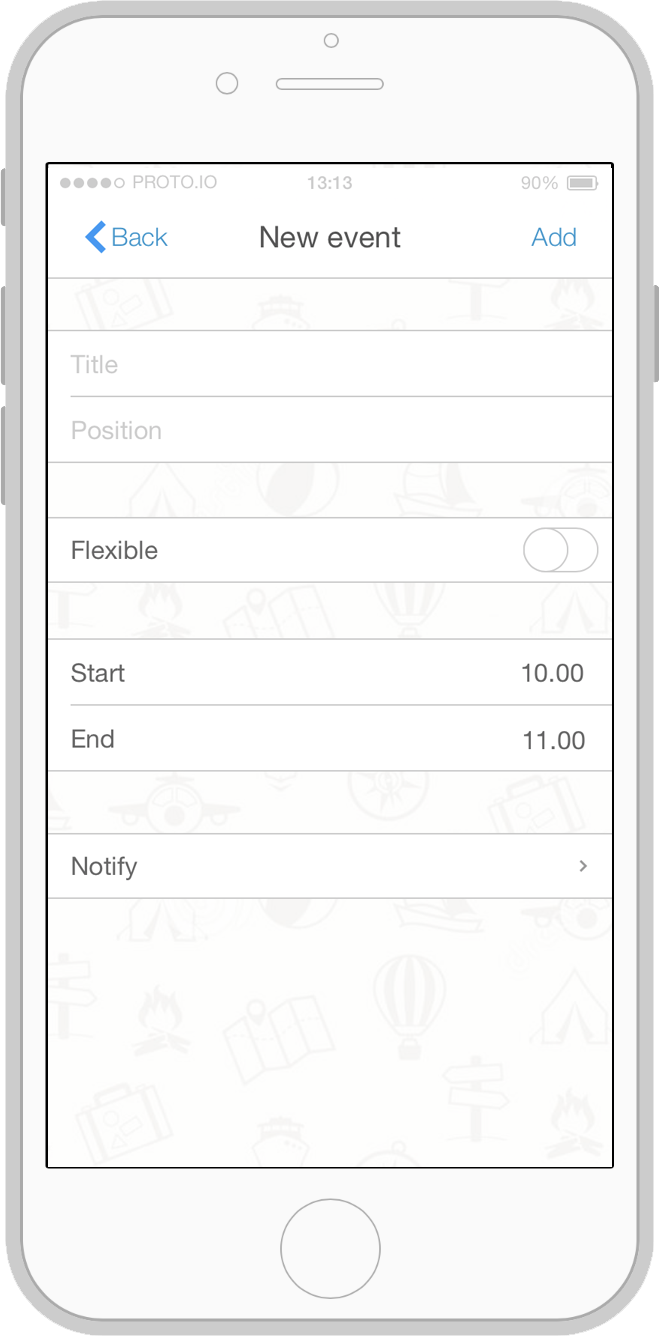
\includegraphics[width=\textwidth]{add_event.png}
		\end{subfigure}
		~
		\begin{subfigure}{0.25\textwidth}
			\centering
			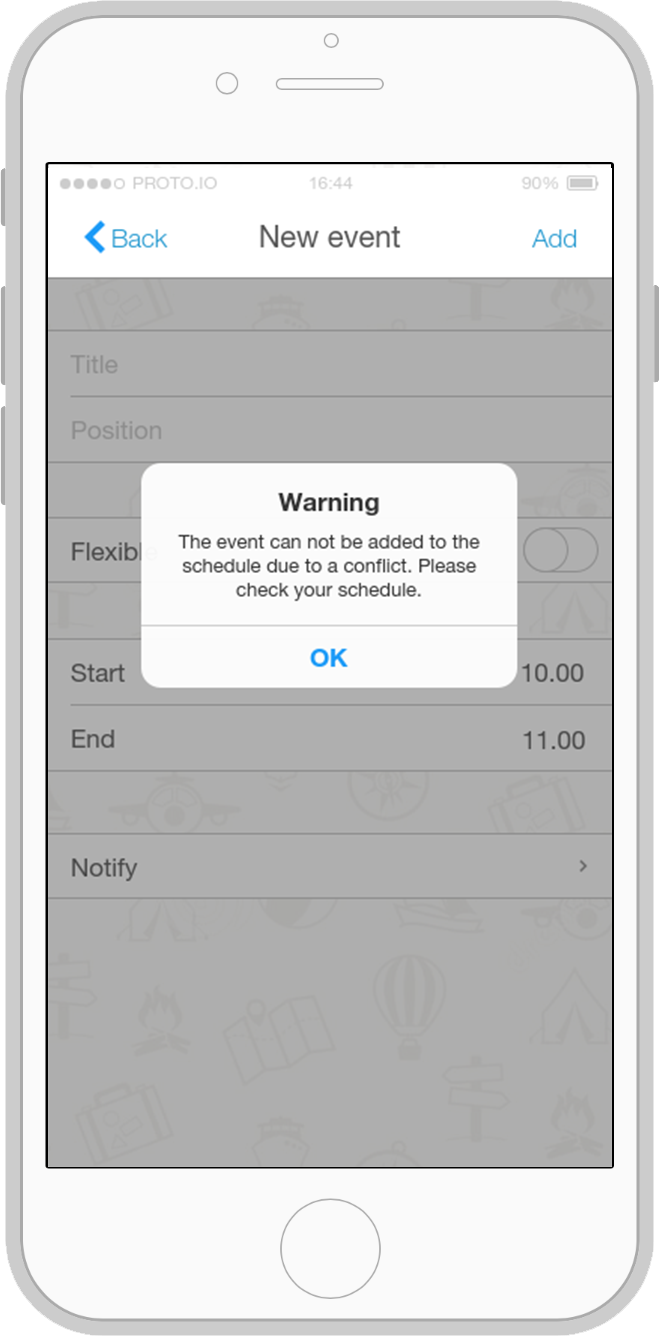
\includegraphics[width=\textwidth]{schedule_conflict.png}
		\end{subfigure}
		~
		\begin{subfigure}{0.25\textwidth}
			\centering
			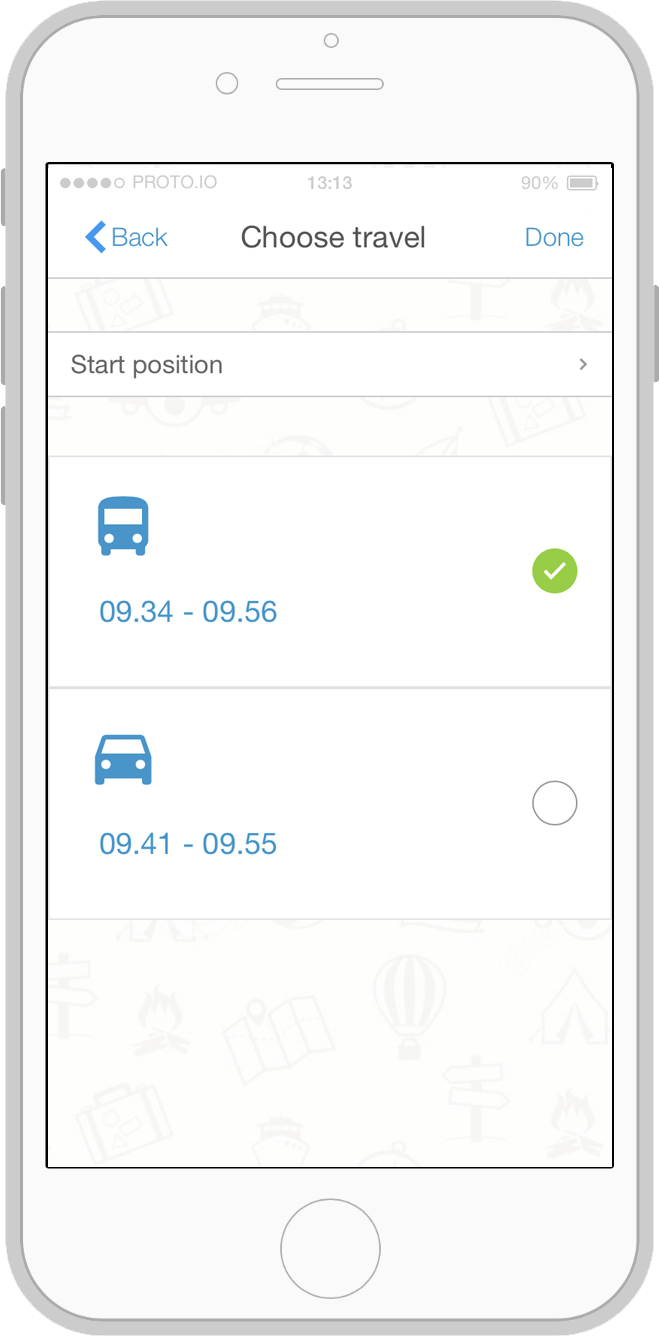
\includegraphics[width=\textwidth]{choose_travel.png}
		\end{subfigure}
	\caption{Add event procedure}
	\end{figure}
%	The User should be able to:
%	\begin{itemize}
%		\item Change the name of the event
%		\item Change the place of the event
%		\item Select the daytime of start and end of the event
%		\item Choose category of the event
%		\item Add a description of the event
%		\item Select the flexibility of the hour of the event: 
%		\item Select possibility for the notification: if is selected, the User should be able to chose when he wants to be notified
%		\item The means of transport selected by the User and the possibility for an "eco" transport
%	\end{itemize}

\end{itemize}
\subsubsection{Hardware Interfaces}
The application is available for mobile devices that guarantee Internet access. The web application can be accessed by any device that provides a reasonably recent browser.

\subsubsection{Software Interfaces}
\begin{itemize}
	\item Operating System: iOS, Android
	\item Web Browser
	\item Web Server application
	\item Development Frameworks
	\item DBMS
	\item Booking System: APIs for third party external services
	\item Mailing System: APIs to send emails to the User
	\item Mapping System: APIs for retrieve transport information
\end{itemize}

\subsubsection{Communication Interfaces}
The application will use HTTPS protocol for communication over the Internet and with the DBMS.

\subsection{Functional Requirements}
In the following section are explained the functional requirements of the application.
\begin{itemize}
	\item \textbf{[R.1]} A visitor must be able to register. During the registration the System will ask to provide credentials.
	\item \textbf{[R.2]} The System must check if the Guest credentials are valid: 
	\begin{itemize}
		\item the username is not already taken by another registered User
		\item the email is in the right format
		\item the password has a minimum length.
	\end{itemize} If credentials are correct, the System sends a confirmation email.
	\item \textbf{[R.3]} The System must store all User data such as personal information, credentials and schedule information.
	\item \textbf{[R.4]} The System must allow the User to log in using his/her personal credentials.
	\item \textbf{[R.5]} The System must allow the User to change username, only if the new username is not already in use by another User, email, only if the new email is in a correct format and password, only if the new password is different from the precedent and respects the minimum length.
	\item \textbf{[R.6]} The System must send a confirmation email if username, email or password is changed. The System must replace the old credentials with the new one.
	\item \textbf{[R.7]} The User must be allowed to create events, specifying:
	\begin{itemize}
		\item The name of the event
		\item The location of the event
		\item The location from which the event will be reached
		\item Start and end date of the event
		\item Start and end time of the event
		\item Notification option
	\end{itemize}
	\item \textbf{[R.8]} The User must be allowed to edit or delete a specific event in his/her schedule.
	\item \textbf{[R.9]} The System allows the User to provide optional event information. This informations are:
	\begin{itemize}
		\item Category type of the event
		\item Brief description of the event
	\end{itemize}
	\item \textbf{[R.10]} The System must allow the User to view all the events for a window of time.
	\item \textbf{[R.11]} The System must check if the event created or edited by the User is feasible.
	\item \textbf{[R.12]} The System must compute travel time between appointments.
	\item \textbf{[R.13]} The System must guarantee a feasible schedule, that is, the User is able to move from an appointment to another in time. The System must warn the User in case of unfeasible event preventing the creation. 
	\item \textbf{[R.14]} The System allows the User to add or edit an event only if it's not in conflict with other events already existent.
	\item \textbf{[R.15]} The System must allow the User to select a specific event.
	\item \textbf{[R.16]} The System must compute the best mobility options taking into account User preferences. If specified, the System must calculate the feasible combination of transportation that minimize carbon footprint.
	\item  \textbf{[R.17]} The System must allow the User to choose one of the mobility option during the event creation and the editing phase of the event.
	\item \textbf{[R.18]} The System allows the User to define specific constraint for each travel means, that are:
	\begin{itemize}
		\item The maximum distance reachable for each mobility option.
		\item The minimum distance of travel necessary for a specific mean of transport to be take into account.
	\end{itemize} 
	\item \textbf{[R.19]} The System must allow the User to be notified a specific time before any event.
	\item \textbf{[R.20]} The System must allow the User to select the \textit{Eco Mode} in order to minimize carbon footprint.
	\item \textbf{[R.21]} The System must allow the User to create flexible events and add additional informations that are:
	\begin{itemize}
		\item Time window in which the event could be created
		\item Duration of the event
	\end{itemize}
	\item \textbf{[R.22]} The System must allow the User to create repetitive events, adding information concerning:
	\begin{itemize}
		\item start/end time
		\item location of the event
		\item frequency of repetition.
	\end{itemize}
	\item \textbf{[R.23]} The System must check the feasibility of flexible events. The System must adapt these events in the schedule only if they are not in conflict with other events already in the schedule. 
	\item \textbf{[R.24]} The System must check the feasibility of repetitive events, taking into account an estimation of the travel time computed at the moment of the creation of the event.
	The System must warn the User in case of conflicts for some of the day specified: the User will be allowed to add the event only in the day with no conflicts or to discard the event creation.
	\item \textbf{[R.25]} For each occurrence of a repetitive event, the User will be allowed to request travel options and choose a travel mean.
	\item \textbf{[R.26]} The System must allow the User to select a specific travel means.
	\item \textbf{[R.27]} The System must provide an interface for third party services allowing the User to authenticate with the service.
	\item \textbf{[R.28]} The System must allow to activate notification and setting its time.
	\item \textbf{[R.29]} The System must activate a ring at the time selected by the User.
\end{itemize}

\subsection{Goals, Requirements and Domain Assumptions}
In the following section functional requirements and domain assumptions are grouped under each goal.
\begin{itemize}
	\item \textbf{[G.1] The System allows the User to access the functionalities of the application from different locations and devices. The data has to be coherent across different devices.}
	\begin{itemize}
		\item [] \textbf{Requirements}
		\item \textbf{[R.1]} A visitor must be able to register. During the registration the System will ask to provide credentials.
		\item \textbf{[R.2]} The System must check if the Guest credentials are valid: 
		\begin{itemize}
			\item the username is not already taken by another registered User
			\item the email is in the right format
			\item the password has a minimum length.
		\end{itemize} If credentials are correct, the System sends a confirmation email.
		\item \textbf{[R.3]} The System must store all User data such as personal information, credentials and schedule information.
		\item \textbf{[R.4]} The System must allow the User to log in using his/her personal credentials.
		\item \textbf{[R.5]} The System must allow the User to change username, only if the new username is not already in use by another User, email, only if the new email is in a correct format and password, only if the new password is different from the precedent and respects the minimum length.
		\item \textbf{[R.6]} The System must send a confirmation email if username, email or password is changed. The System must replace the old credentials with the new one.
		\item [] \textbf{Domain assumptions}
		\item \textbf{[D.1]} The given email is assumed to be correct.
		\item \textbf{[D.2]} The sent mail is assumed to be correctly received.
		\item \textbf{[D.3]} The Storage System is reliable.
	\end{itemize}

	\item \textbf{[G.2] The System allows the User to manage meetings in his/her schedule.}
	\begin{itemize}
		\item [] \textbf{Requirements}
		\item \textbf{[R.4]}The System must allow the User to log in using his/her personal credentials.
		\item \textbf{[R.7]} The User must be allowed to create events, specifying:
		\begin{itemize}
			\item The name of the event
			\item The location of the event
			\item The location from which the event will be reached
			\item Start and end date of the event
			\item Start and end time of the event
			\item Notification option
		\end{itemize}
		\item \textbf{[R.8]} The User must be allowed to edit or delete a specific event in his/her schedule.
		\item \textbf{[R.9]} The System allows the User to provide optional event information. This informations are:
		\begin{itemize}
			\item Category type of the event
			\item Brief description of the event
		\end{itemize}
		\item \textbf{[R.10]} The System must allow the User to view all the events for a window of time.
		\item \textbf{[R.11]} The System must check if the event created or edited by the User is feasible.
		\item [] \textbf{Domain assumptions}
		\item \textbf{[D.3]} The events informations provided by the user are correct.
	\end{itemize}

	\item \textbf{[G.3] The System allows the User to reach every meeting on time.}
	\begin{itemize}
		\item [] \textbf{Requirements}
		\item \textbf{[R.12]} The System must compute travel time between appointments.
		\item \textbf{[R.13]} The System must guarantee a feasible schedule, that is, the User is able to move from an appointment to another in time. The System must warn the User in case of unfeasible event preventing the creation. 
		\item \textbf{[R.14]} The System allows the User to add or edit an event only if it's not in conflict with other events already existent.
		\item [] \textbf{Domain assumptions}
		\item\textbf{[D.4]} Event time constraint are respected by the User.
		\item \textbf{[D.5]} The informations about the event are correct.
	\end{itemize}

	\item \textbf{[G.4] The System allows the User to select or edit a travel means to reach an event.}
	\begin{itemize}
		\item[] \textbf{Requirements}
		\item \textbf{[R.15]} The System must allow the User to select a specific event.
		\item \textbf{[R.16]} The System must compute the best mobility options taking into account User preferences. If specified, the System must calculate the feasible combination of transportation that minimize carbon footprint.
		\item  \textbf{[R.17]} The System must allow the User to choose one of the mobility option during the event creation and the editing phase of the event.
		\item[] \textbf{Domain assumptions}
		\item \textbf{[D.6]} The informations about available mobility options and related travel time are correct.
		\item \textbf{[D.7]} If selected, the private means of transport are available without any delay.
		\item \textbf{[D.8]} The start location of the travel is known and correct.
	\end{itemize} 

	\item \textbf{[G.5] The System allows the User to set preferences.}
	\begin{itemize}
		\item [] \textbf{Requirements}
		\item \textbf{[R.4]} The System must allow the User to login using his/her personal credentials.
		\item \textbf{[R.18]} The System allows the User to define specific constraint for each travel means, that are:
		\begin{itemize}
			\item The maximum distance reachable for each mobility option.
			\item The minimum distance of travel necessary for a specific mean of transport to be take into account.
		\end{itemize} 
		\item \textbf{[R.19]} The System must allow the User to be notified a specific time before any event.
		\item \textbf{[R.20]} The System must allow the User to select the \textit{Eco Mode} in order to minimize carbon footprint.
		\item [] \textbf{Domain assumption}
		\item \textbf{[D.9]} All selected travel means specified in the preferences are potentially available to the User.
		\item \textbf{[D.10]} A minimum walking distance is assumed in order to reach every mean of transport. Such distance will not be taken into account unless significant with respect to the travel time, meaning unless it influences the ETA by more than a minute.
	\end{itemize}

	\item \textbf{[G.6]} The System allows the User to create flexible events and repetitive events.
	\begin{itemize}
		\item [] \textbf{Requirements}
		\item \textbf{[R.4]} The System must allow the User to login using his/her personal credentials.
		\item \textbf{[R.21]} The System must allow the User to create flexible events and add additional informations that are:
		\begin{itemize}
			\item Time window in which the event could be created
			\item Duration of the event
		\end{itemize}
		\item \textbf{[R.22]} The System must allow the User to create repetitive events, adding information concerning:
		\begin{itemize}
			\item start/end time
			\item location of the event
			\item frequency of repetition.
		\end{itemize}
		\item \textbf{[R.23]} The System must check the feasibility of flexible events. The System must adapt these events in the schedule only if they are not in conflict with other events already in the schedule. 
		\item \textbf{[R.24]} The System must check the feasibility of repetitive events, taking into account an estimation of the travel time computed at the moment of the creation of the event.
		The System must warn the User in case of conflicts for some of the day specified: the User will be allowed to add the event only in the day with no conflicts or to discard the event creation.
		\item \textbf{[R.25]} For each occurrence of a repetitive event, the User will be allowed to request travel options and choose a travel mean.
		\item [] \textbf{Domain assumption}
		\item\textbf{[D.4]} Event time constraint are respected by the User.
	\end{itemize}

	\item \textbf{[G.7] The System allows the User to book transportation for a travel.}
	\begin{itemize}
		\item [] \textbf{Requirements}
		\item \textbf{[R.4]} The System must allow the User to login using his/her personal credentials.
		\item \textbf{[R.26]} The System must allow the User to select a specific travel means.
		\item \textbf{[R.27]} The System must provide an interface for third party services allowing the User to authenticate with the service.
		\item [] \textbf{Domain assumptions}
		\item \textbf{[D.11]} The User is registered to the service which offers the booking option.
	\end{itemize}

	\item \textbf{[G.8] The System allows the User to be notified before the occurrence of an event.}
	\begin{itemize}
		\item [] \textbf{Requirements}
		\item \textbf{[R.4]} The System must allow the User to login using his/her credentials.
		\item \textbf{[R.28]} The System must allow to activate notification and setting its time.
		\item \textbf{[R.29]} The System must activate a ring at the time selected by the User.
		\item [] \textbf{Domain assumptions}
		\item \textbf{[D.12]} The System internal clock time used to provide notifications is correct.
	\end{itemize}
\end{itemize}

\subsection{Performance Requirements}
\textit{Travlendar+} is structured in a three-tier architecture. All the application logic is built in the application servers: the backend performances should guarantee the proper operation in case of traffic peaks and manage multiple Users.

\subsection{Design Constraints}
\subsubsection{Standards Compliance}
All Informations concerning locations are given in form of Latitude and Longitude degrees. 

\subsubsection{Hardware Limitations}
The application should be able to run, at least, under the following conditions:
\begin{itemize}
	\item 3G connections at 2Mb/s
	\item 50 MB of space
	\item 2 GB of RAM
\end{itemize}

\subsection{Software Attributes}

\subsubsection{Reliability}
The System should guarantees a $99\%$ of reliability: its components must have a failure rate that guarantees this goal.

\subsubsection{Availability}
The System guarantees an high availability, due to the expected high reliability, in order to offer an ideal 24/7 service.

\subsubsection{Security}
User credentials and data will be stored in a DBMS that should guarantee an high security. For what concerns the User credential, in order to provide this result, the passwords stored in the DBMS are salted and hashed.\\
As already mentioned, the System uses HTTPS protocol to communicate with all the services, in order to guarantee protection of the privacy and integrity of the exchanged data.\\
The payment security for the booking functionality is guaranteed by third-party services and the System is not responsible in case of damage. 

\subsubsection{Maintainability}
The System will have a modular architecture: each component is organized in a hierarchical way in order to speed up the maintenance in case of failure. This structure is also convenient for further refinements of single components.

\subsubsection{Portability}
The application is developed in terms of Web Application and native application for iOS and Android. Furthermore, the three-tier architecture of the System allows to define a backend in which all the business logic is built, ensuring an high level of portability.


\newpage
\section{Formal Analysis Using Alloy}
In this section a model of the World is provided by the Alloy tool.
\subsection{Model}

\begin{lstlisting}[language=alloy]
open util/boolean

---------------- AVAILABLE PREFERENCES ----------------

sig publicPreference extends Preference {
maxCost : Int,
maxChanges : Int
} { maxCost > 0 and maxChanges >= 0}

sig footPreference extends Preference {
maxDistance: Int
} {maxDistance > 0}

sig bikePreference extends Preference {
maxDistance: Int
} {maxDistance > 0}

sig taxiPreference extends Preference {
maxCost: Int
} {maxCost > 0}

sig carPreference extends Preference {
minDistance: Int
} {minDistance > 0}

sig bikeSharingPreference extends Preference {
maxDistance: Int,
maxCost: Int
} {maxCost > 0 and maxDistance > 0}

sig carSharingPreference extends Preference {
minDistance: Int,
maxCost: Int
} {maxCost > 0 and minDistance > 0}

---------------- AVAILABLE TRANSPORTS ----------------

-- an instance of transport is intended as additional information about a specific travel once the type of mean is defined

sig Foot extends Transport {
distance : Int
} { distance > 0 }

sig Taxi extends Transport {
cost : Int
} { cost > 0 }

sig Car extends Transport {
distance : Int
} { distance > 0 }

sig Public extends Transport {
cost : Int,
nChanges: Int
} { cost > 0 and nChanges >= 0}

sig Bike extends Transport {
distance : Int
} { distance > 0 }

sig carSharing extends Transport {
distance: Int,
cost: Int
} { cost > 0 and distance > 0}

sig bikeSharing extends Transport  {
distance,
cost: Int,
} { cost > 0 and distance > 0}

---------------- MODEL SIGNATURES ----------------

abstract sig Preference {}
abstract sig Transport {}

sig Booking {}

sig User {
calendar: set Schedule,
constraints: set Preference,
id: one Int
} { id > 0 }

sig Schedule {
scheduleEvents: set Event,
scheduleTravels: set Travel
} { 
-- each schedule has 1 starting event i.e. no travel has this event as a destination
-- and 1 final event i.e. no travel has this event as a source, these events can coincide.
-- all other events are connected by travels
(one e: scheduleEvents | no t: scheduleTravels | t.to = e)	and (one e: scheduleEvents | no t: scheduleTravels | t.from = e)
}

sig Event {
start: one Int,
end: one Int,
active: one Bool
} { start > 0 and end > 0 and start < end }

sig Travel {
from: one Event,
to: one Event,
start: one Int,
end: one Int,
mean: one Transport,
travelBooking: lone Booking
} { start > 0 and end > 0 and start < end}

-- each preference is in the constraints of 1 user
fact eachPreferenceBelongsToAUser {
all p: Preference | one u: User  | p in u.constraints
}

-- the id associated with each user is unique
fact userIdsAreUnique {
no disjoint u1, u2 : User | u1.id = u2.id
}

-- each users can specify one constraint/preference of each type
fact userHasOnePreferencePerType {
all u: User {
lone p: Preference | p in bikePreference and p in u.constraints
lone p: Preference | p in footPreference and p in u.constraints
lone p: Preference | p in publicPreference and p in u.constraints
lone p: Preference | p in bikeSharingPreference and p in u.constraints
lone p: Preference | p in carSharingPreference and p in u.constraints
lone p: Preference | p in carPreference and p in u.constraints
lone p: Preference | p in taxiPreference and p in u.constraints
}
}

-- the preferences of each user must be respected in the model
fact preferencesMustBeRespected {
no u: User {
all s: Schedule {
all t: Travel {
some p: publicPreference, pt: Public | pt.nChanges > p.maxChanges and p in u.constraints and t in s.scheduleTravels and t.mean = pt
some p: publicPreference, pt: Public | pt.cost > p.maxCost and p in u.constraints and t in s.scheduleTravels and t.mean = pt
some p: footPreference, ft: Foot | ft.distance > p.maxDistance and p in u.constraints and t in s.scheduleTravels and t.mean = ft
some p: bikePreference, bt : Bike | bt.distance > p.maxDistance and p in u.constraints and t in s.scheduleTravels and t.mean = bt
some p: taxiPreference, tt: Taxi | tt.cost > p.maxCost and p in u.constraints and t in s.scheduleTravels and t.mean = tt
some p: carPreference, ct : Car | ct.distance < p.minDistance and p in u.constraints and t in s.scheduleTravels and t.mean = ct
some p: carSharingPreference, st : carSharing | st.cost > p.maxCost and p in u.constraints and t in s.scheduleTravels and t.mean = st
some p: carSharingPreference, st : carSharing | st.distance < p.minDistance and p in u.constraints and t in s.scheduleTravels and t.mean = st
some p: bikeSharingPreference, st : bikeSharing | st.distance > p.maxDistance and p in u.constraints and t in s.scheduleTravels and t.mean = st
some p: bikeSharingPreference, st : bikeSharing | st.cost > p.maxCost and p in u.constraints and t in s.scheduleTravels and t.mean = st
}
}
}
}

-- each schedule is in the calendar of 1 user
fact eachScheduleBelongsToAUser {
all s:Schedule | one u: User | s in u.calendar
}

-- each active event is in 1 schedule
fact eachEventBelongsToASchedule {
all e: Event | one s: Schedule | e in s.scheduleEvents or (e.active = False and not e in s.scheduleEvents)
}

-- booking is available for public transportation, taxi and sharing services
fact bookingServices {
all t: Travel | all b : Booking | t.travelBooking = b implies t.mean in Taxi + Public + carSharing + bikeSharing
}

-- each travel is in 1 schedule
fact eachTravelBelongsToASchedule {
all t: Travel | one s: Schedule | t in s.scheduleTravels
}

-- each booking referes to 1 travel
fact eachBookingBelongsToATravel {
all b: Booking | one t: Travel | t.travelBooking = b
}

-- each instance of transport is associated with a travel 
fact eachTransportBelongsToATravel {
all tt: Transport | one t: Travel | t.mean = tt
}

-- inactive events do not belong in any schedule
fact inactiveEventsdoNotBelongInAnySchedule {
all s: Schedule | all e: Event | e in s.scheduleEvents implies e.active = True
}

-- for any given travel there are 2 events, source and destination
-- that respectively end before the start of the travel and start after the start of the travel
fact travelIsBetweenEventsTimes {
no t: Travel | t.start < t.from.end or t.end > t.to.start
}

-- each travel must have a source and a destination
fact travelHasToAndFrom {
all t: Travel | some disjoint e1, e2: Event | t.to = e1 and t.from = e2
}

-- no travel can connect events from 2 different schedule
fact noTravelAcrossSchedules {
all t: Travel | all s: Schedule | t.to in s.scheduleEvents implies t.from in s.scheduleEvents and t in s.scheduleTravels
}

-- no travel can connect to or from inactive events
fact noTravelToOrFromInactive {
no t: Travel | t.from.active = False or t.to.active = False
}

-- this means that the instances of the transport are different not the type of transport
fact differentTravelHaveDifferentMean {
no disjoint t1, t2 : Travel | t1.mean = t2.mean
}

-- for each 2 events the start or end time can not coincide
fact scheduleEventsDoNotEndOrStartAtTheSameTime {
all s: Schedule | all disjoint e1, e2: Event | 
(e1 in s.scheduleEvents and e2 in s.scheduleEvents) implies (e1.start != e2.start and e1.end != e2.end)
}

-- events do not intersect
fact noIntersectingEvents {
all s: Schedule | all disjoint e1, e2: Event | 
(e1 in s.scheduleEvents and e2 in s.scheduleEvents and e1.start < e2.start) implies e1.end < e2.start
}

-- there is only one travel that has a certain event as source or as a destination
fact noDoubleTravelPerEvent {
no disjoint t1, t2 : Travel | t1.from = t2.from or  t1.to = t2.to
}
---------------- ASSERTIONS ----------------

-- the event that is not the destination of any travel (starting
assert noEventBeforeFirstAndAfterLastEvent {
all s: Schedule | no disjoint e1, e2 : Event | 
isFirstOfSchedule[e1,s] and e2.start < e1.end and e2 + e1 in s.scheduleEvents or
isLastOfSchedule[e1,s] and e2.end > e1.start and e2 + e1 in s.scheduleEvents
}

-- there are no intersection between schedules in terms of travels and events
assert allSchedulesAreDisjoint {
all disjoint s1, s2: Schedule | no e: Event, t:Travel | (e in s1.scheduleEvents and e in s2.scheduleEvents) 
or (t in s1.scheduleTravels and t in s2.scheduleTravels)
}

-- a travel only connects events in chronological order
assert cannotTravelInThePast{
all s: Schedule | all t: Travel | no e1, e2: Event | (e1+e2 in s.scheduleEvents and t.to = e1 and t.from = e2)
and (e2.end > e1.start)
}

---------------- PREDICATES ----------------

pred show {}

pred isLastOfSchedule[e: Event, s: Schedule] {
no t : Travel | t.from = e and e in s.scheduleEvents and t in s.scheduleTravels
}

pred isFirstOfSchedule[e: Event, s: Schedule] {
no t : Travel | t.to = e and e in s.scheduleEvents and t in s.scheduleTravels
}

pred addEvent[e: Event, s: Schedule] {
s.scheduleEvents = s.scheduleEvents + e
}

pred addBooking[t, t': Travel, new_b: Booking, s: Schedule] {
t'.travelBooking = new_b
t'.from = t.from
t'.to = t.to
t'.start = t.start
t'.end = t.end
t'.mean = t.mean
s.scheduleTravels = s.scheduleTravels - t + t'
t + t' in s.scheduleTravels
}

pred changeEventTime[e, e' : Event, s: Schedule, new_end, new_start : Int] {
e'.start = new_start
e'.end = new_end
e'.active = e.active
s.scheduleEvents = s.scheduleEvents - e + e'
}

pred changeTravelTransport[t, t': Travel, s: Schedule, new_mean: Transport] {
t'.travelBooking = t.travelBooking
t'.from = t.from
t'.to = t.to
t'.start = t.start
t'.end = t.end
t'.mean = new_mean
s.scheduleTravels = s.scheduleTravels - t + t'
t + t' in s.scheduleTravels
}

---------------- CHECK ASSERTIONS ----------------

check noEventBeforeFirstAndAfterLastEvent for  10 Event, 10 Travel, 10 User, 10 Schedule, 10 Transport, 10 Booking, 6 Preference, 4 Int
check allSchedulesAreDisjoint for  10 Event, 10 Travel, 10 User, 10 Schedule, 10 Transport, 10 Booking, 6 Preference, 4 Int
check cannotTravelInThePast for  10 Event, 10 Travel, 10 User, 10 Schedule, 10 Transport, 10 Booking, 6 Preference, 4 Int

---------------- RUN PREDICATES ----------------

run show for exactly 4 Event, 10 Travel, 2 User, 2 Schedule, 10 Transport, 2 Booking,  5 Preference, 4 Int
run addBooking for 10 Event, 10 Travel, 2 User, 2 Schedule, 10 Transport, 2 Booking,  5 Preference, 4 Int
run addEvent for 10 Event, 10 Travel, 2 User, 2 Schedule, 10 Transport, 2 Booking,  5 Preference, 4 Int
run changeEventTime for 10 Event, 10 Travel, 2 User, 2 Schedule, 10 Transport, 2 Booking,  5 Preference, 4 Int
run changeTravelTransport for 10 Event, 10 Travel, 2 User, 2 Schedule, 10 Transport, 2 Booking,  5 Preference, 4 Int

\end{lstlisting}

\subsection{Model Checks}

\begin{figure}[H]
	\centering
	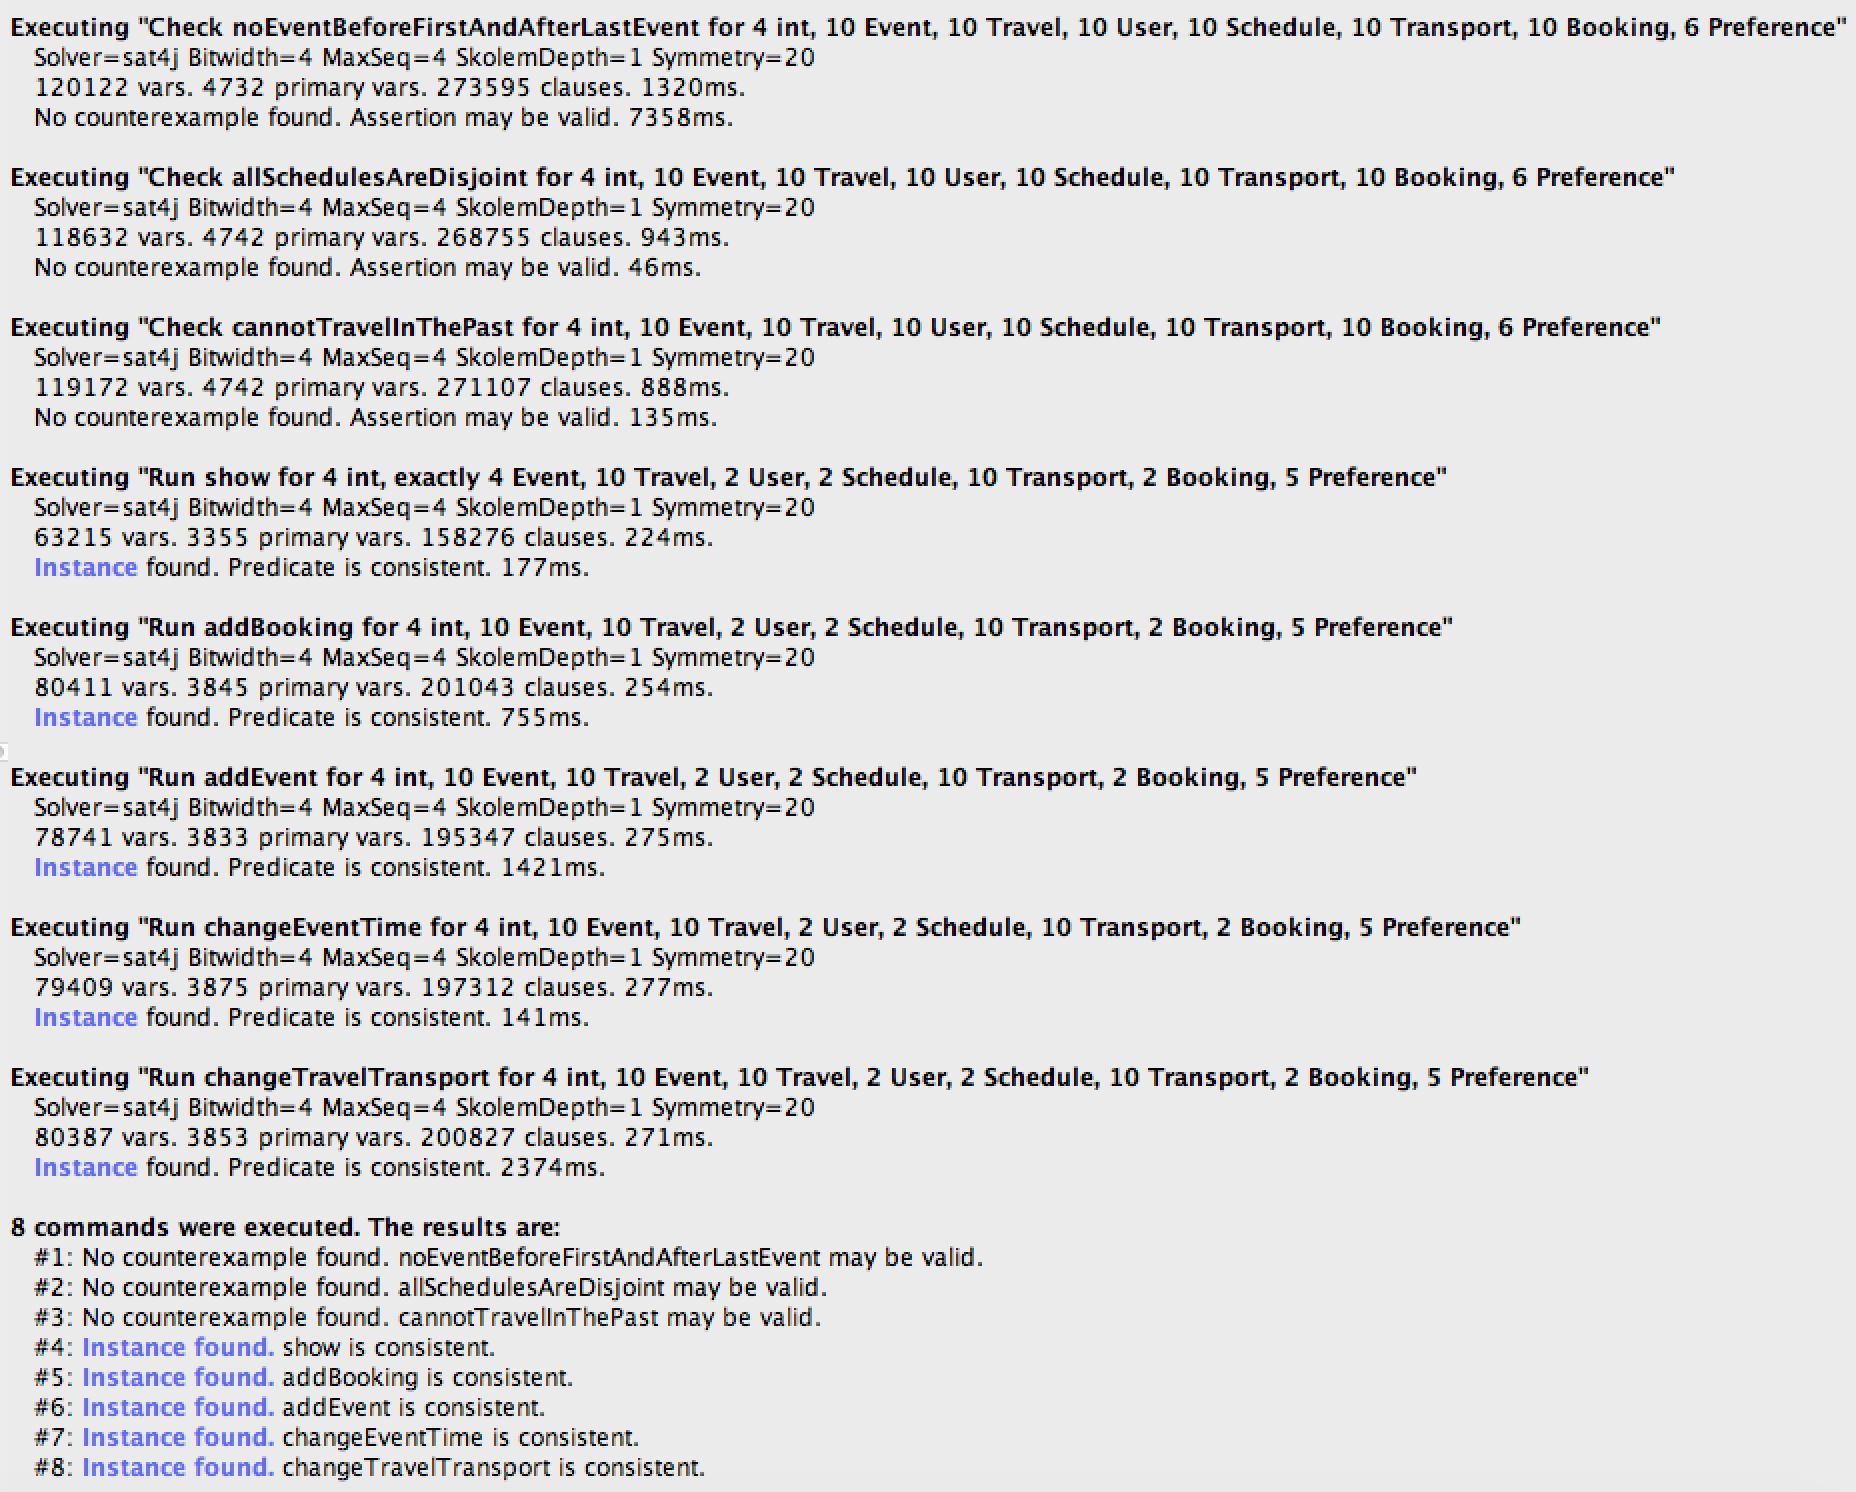
\includegraphics[width=1\textwidth]{res_alloy}
\end{figure}

\newpage

\subsection{Generated Worlds}

\begin{lstlisting}[language=alloy]
pred show {
#Schedule = 1
#User = 1
#Preference = 1
#Booking = 0
}

run show for exactly 2 Event, 10 Travel, 2 User, 3 Schedule, 10 Transport, 2 Booking,  5 Preference, 4 Int
\end{lstlisting}

\begin{figure}[H]
	\centering
	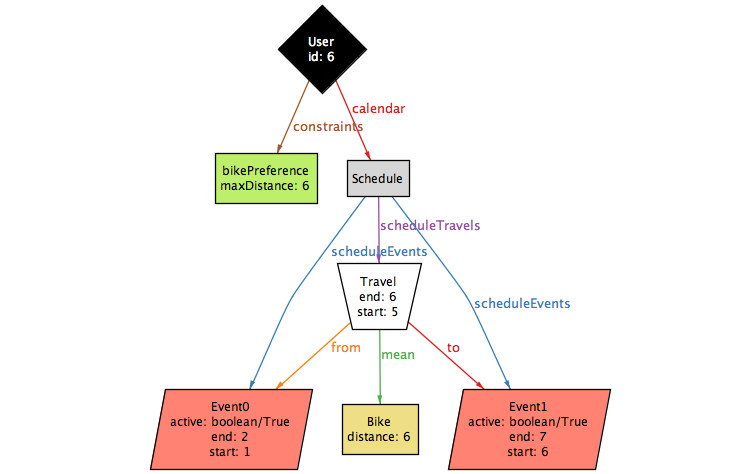
\includegraphics[width=1\textwidth]{world_show_3}
\end{figure}
\newpage
\begin{lstlisting}[language=alloy]
pred show {
#Schedule = 3
#User = 1
#Preference = 2
#Booking = 1
}

run show for exactly 6 Event, 10 Travel, 2 User, 3 Schedule, 10 Transport, 2 Booking,  5 Preference, 4 Int
\end{lstlisting}

\begin{figure}[H]
	\centering
	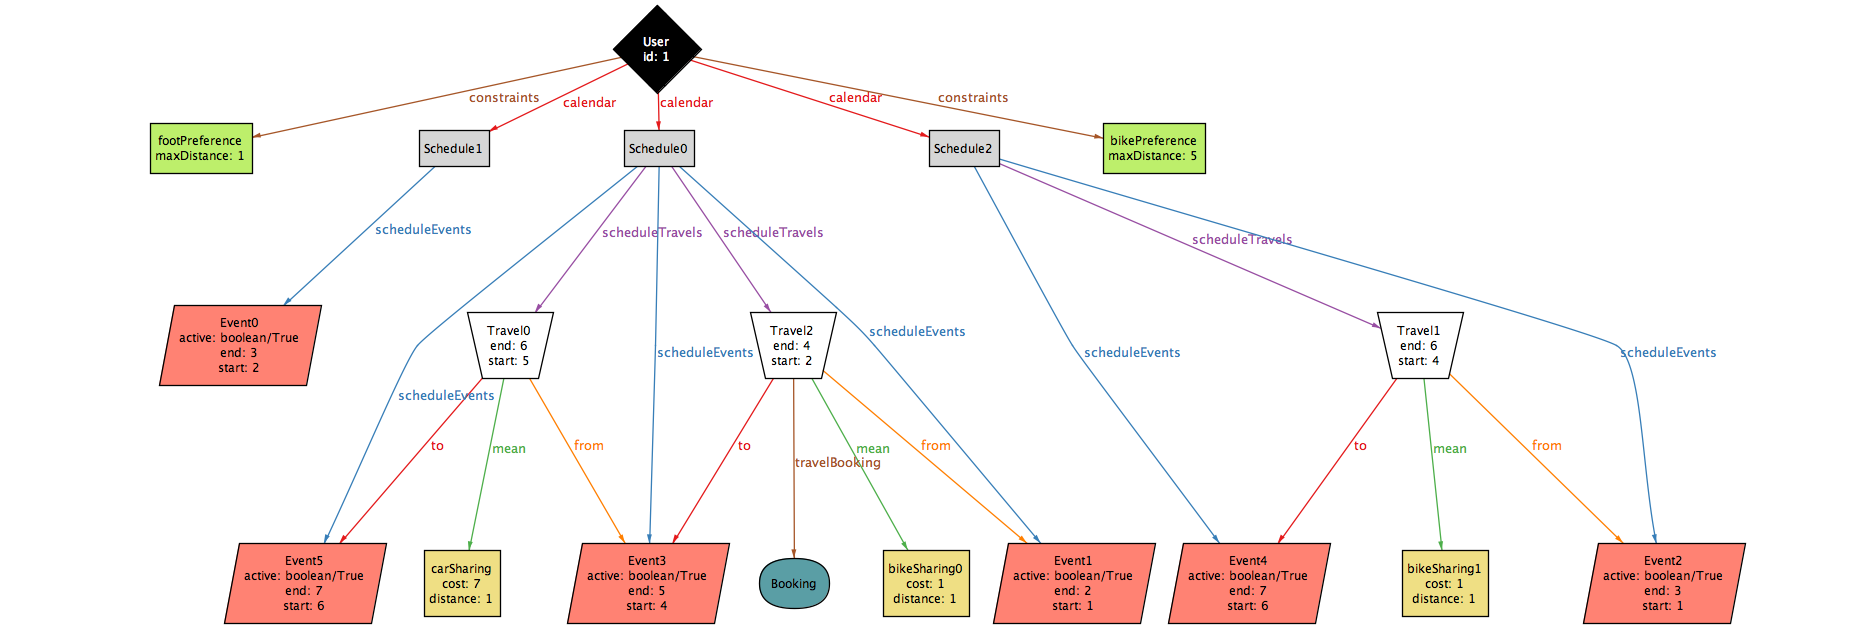
\includegraphics[width=1\textwidth]{world_show_2}
\end{figure}

\begin{lstlisting}[language=alloy]
pred show {
#Schedule = 2
#User = 2
#Preference = 4
#Booking = 1
}

run show for exactly 6 Event, 10 Travel, 2 User, 2 Schedule, 10 Transport, 2 Booking,  5 Preference, 4 Int
\end{lstlisting}

\begin{figure}[H]
	\centering
	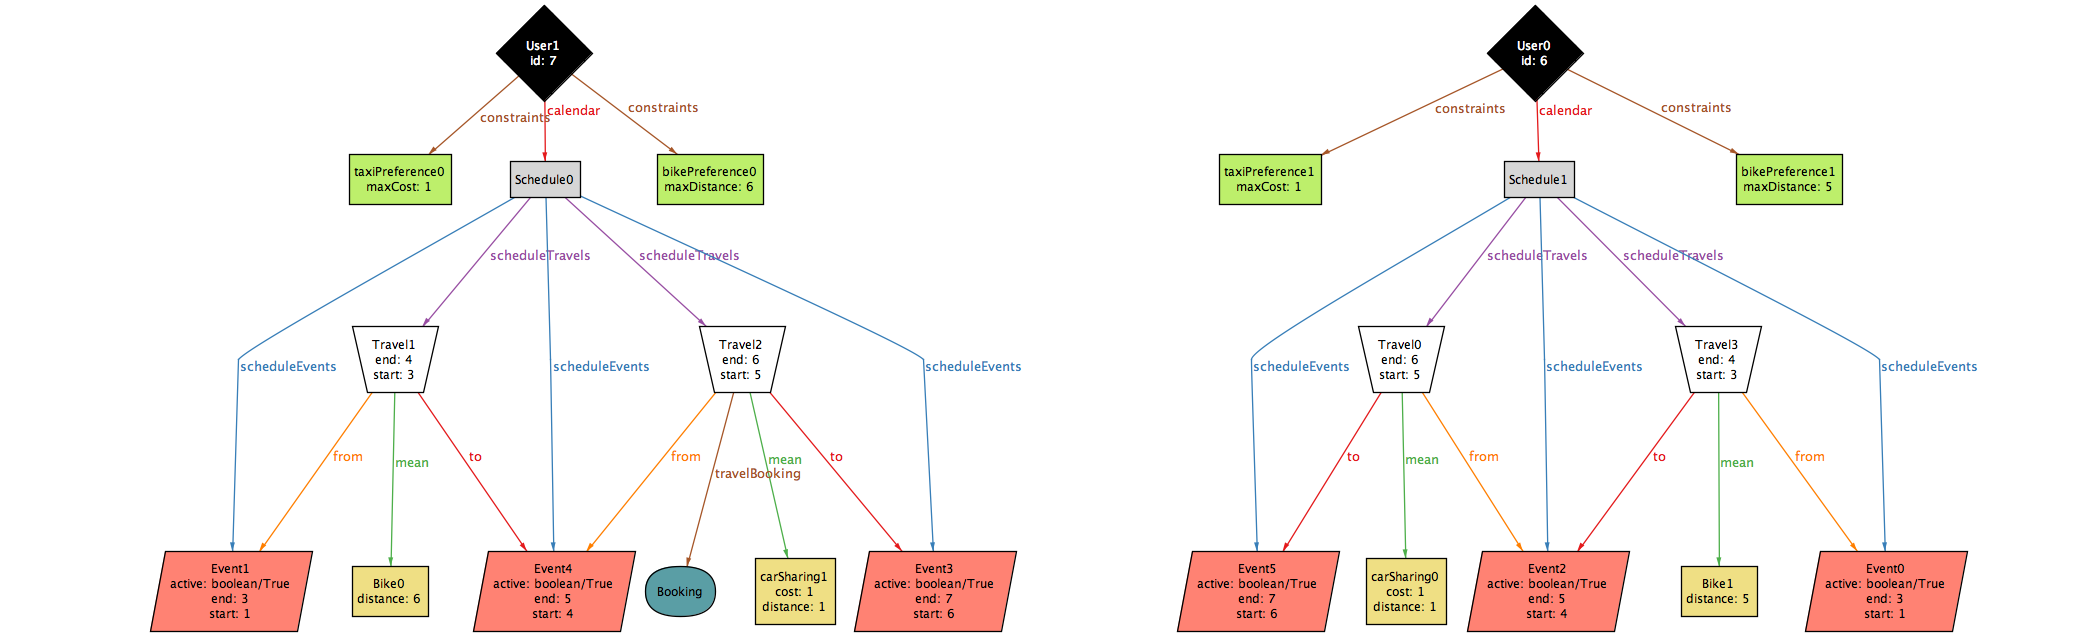
\includegraphics[width=1\textwidth]{world_show_1}
\end{figure}


\begin{lstlisting}[language=alloy]
pred addEvent[e: Event, s: Schedule] {
s.scheduleEvents = s.scheduleEvents + e
}

run addEvent for 10 Event, 10 Travel, 2 User, 2 Schedule, 10 Transport, 2 Booking,  5 Preference, 4 Int
\end{lstlisting}

\begin{figure}[H]
	\centering
	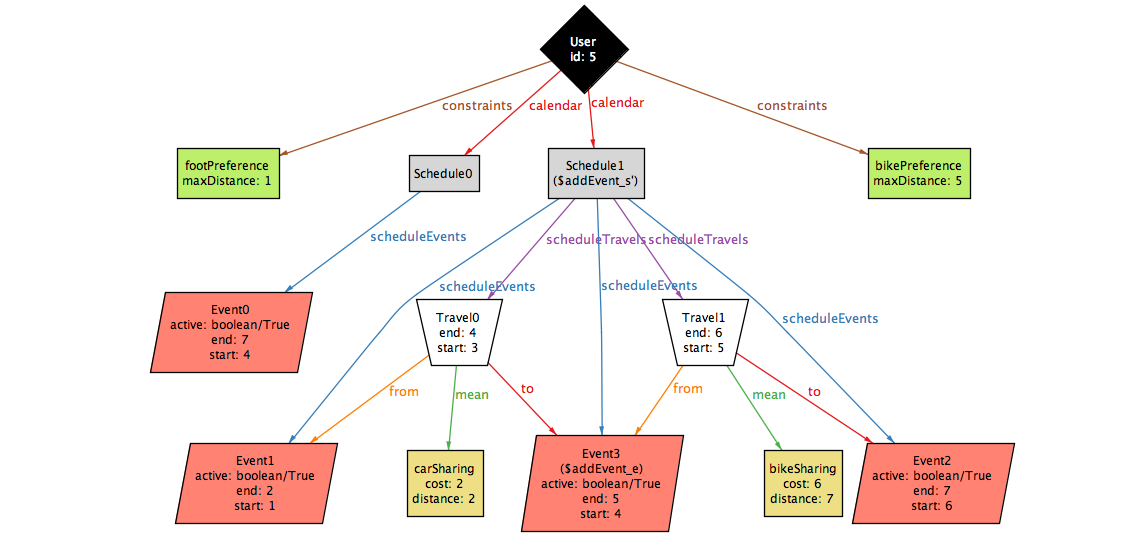
\includegraphics[width=1\textwidth]{world_add_event}
\end{figure}

\begin{lstlisting}[language=alloy]
pred addBooking[t, t': Travel, new_b: Booking, s: Schedule] {
t'.travelBooking = new_b
t'.from = t.from
t'.to = t.to
t'.start = t.start
t'.end = t.end
t'.mean = t.mean
s.scheduleTravels = s.scheduleTravels - t + t'
t + t' in s.scheduleTravels
}

run addBooking for 10 Event, 10 Travel, 2 User, 2 Schedule, 10 Transport, 2 Booking,  5 Preference, 4 Int
\end{lstlisting}

\begin{figure}[H]
	\centering
	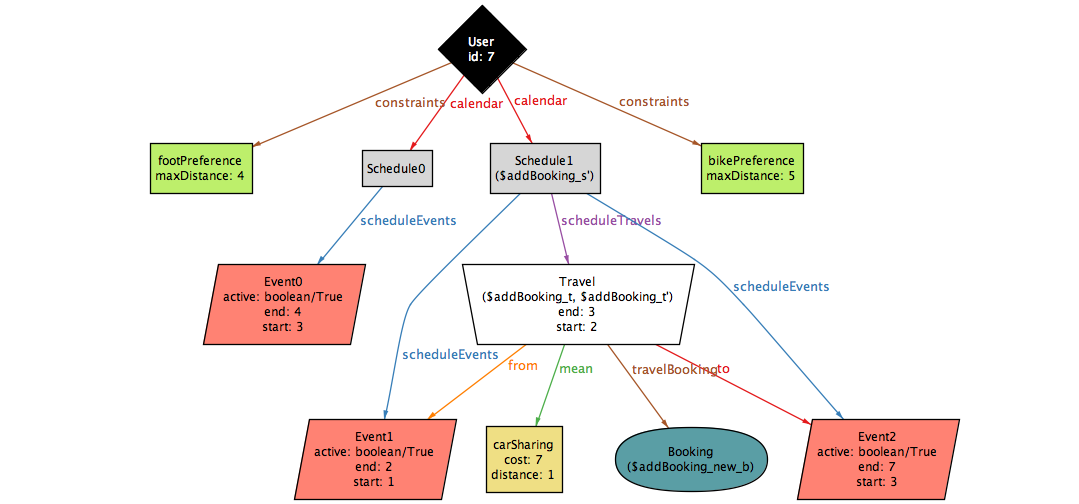
\includegraphics[width=1\textwidth]{world_add_booking}
\end{figure}

\begin{lstlisting}[language=alloy]
pred changeEventTime[e, e' : Event, s: Schedule, new_end, new_start : Int] {
e'.start = new_start
e'.end = new_end
e'.active = e.active
s.scheduleEvents = s.scheduleEvents - e + e'
e + e' in s.scheduleEvents
}

run changeEventTime for 10 Event, 10 Travel, 2 User, 2 Schedule, 10 Transport, 2 Booking,  5 Preference, 4 Int
\end{lstlisting}

\begin{figure}[H]
	\centering
	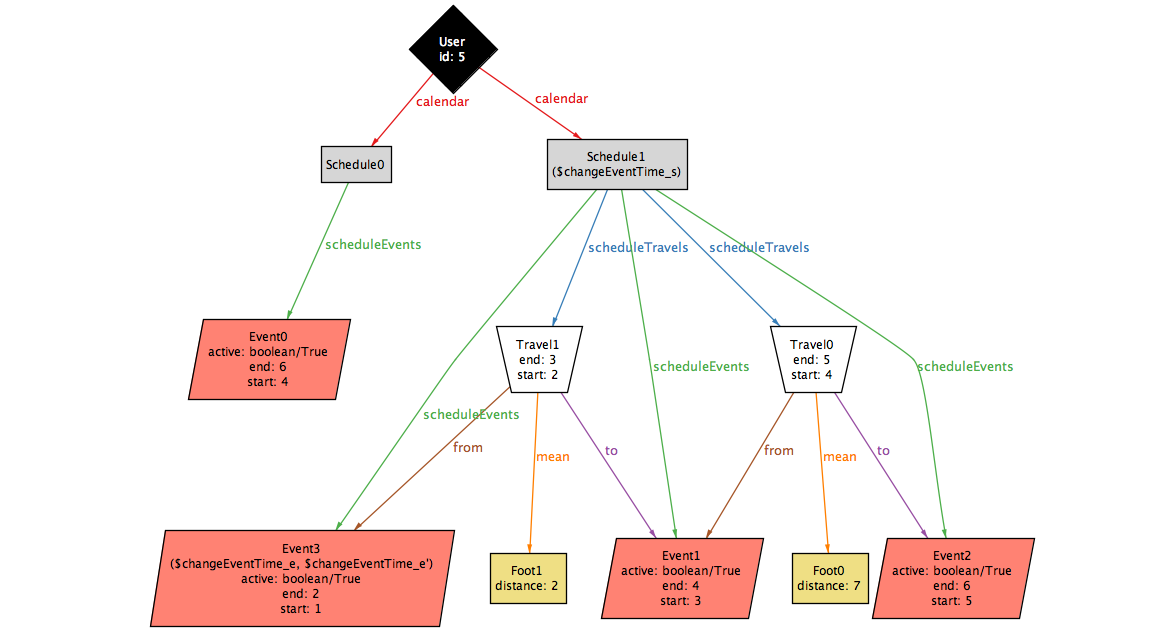
\includegraphics[width=1\textwidth]{world_change_event_time}
\end{figure}


\begin{lstlisting}[language=alloy]
pred changeTravelTransport[t, t': Travel, s: Schedule, new_mean: Transport] {
t'.travelBooking = t.travelBooking
t'.from = t.from
t'.to = t.to
t'.start = t.start
t'.end = t.end
t'.mean = new_mean
s.scheduleTravels = s.scheduleTravels - t + t'
t + t' in s.scheduleTravels
}

run changeTravelTransport for 10 Event, 10 Travel, 2 User, 2 Schedule, 10 Transport, 2 Booking,  5 Preference, 4 Int
\end{lstlisting}

\begin{figure}[H]
	\centering
	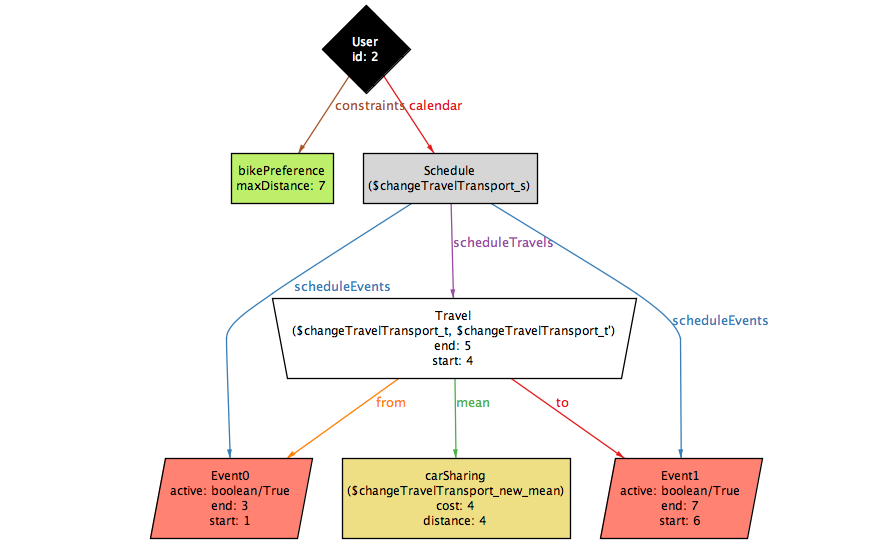
\includegraphics[width=1\textwidth]{world_change_travel_transport}
\end{figure}
\newpage
\section{Effort Spent}

The effort spent from each member of the team to build the RASD can be summarized as follow: \\

\noindent
\textbf{Guglielmo Menchetti}\\

\begin{tabular}{| l | l | l |}
	\hline
	\textbf{Date} & \textbf{Task} & \textbf{Hours}\\
	\hline
	02/10/17 & First meeting & 4\\
	03/10/17 & Github setup & 1,5\\
	04/10/17 & Purpose and Scope & 3,5 \\
	06/10/17 & Product Functions & 2,5 \\
	09/10/17 & Design Constraints & 2 \\
	10/10/17 & Mapping Goals and Functional Requirements & 4,5 \\
	12/10/17 & Goals review & 2,5 \\
	14/10/17 & External Interface Requirements & 2 \\
	15/10/17 & Mid-phase meeting & 3,5 \\
	19/10/17 & Software Attributes & 1,5 \\
	20/10/17 & Requirements review & 2,5 \\
	22/10/17 & Domain Assumptions list & 3 \\
	23/10/17 & Introduction review & 3 \\
	24/10/17 & Alloy and Requirements & 4\\
	26/10/17 & Global review & 4 \\
	27/10/17 & Alloy refinements & 3\\
	\hline
	& & \textbf{Total}\\
	\hline
	& & 47\\	
	\hline

\end{tabular}\\

\newpage
\noindent
\textbf{Lorenzo Norcini}\\

\begin{tabular}{| l | l | l |}
	\hline
	\textbf{Date} & \textbf{Task} & \textbf{Hours}\\
	\hline
	02/10/17 & First meeting & 4\\
	03/10/17 & Github setup & 1,5\\
	04/10/17 & Purpose and Scope & 3,5 \\
	07/10/17 & Class Diagram & 2,5 \\
	09/10/17 & Performance Requirements & 1,5\\
	10/10/17 & Mapping Goals and Functional Requirements & 4,5 \\
	11/10/17 & State Chart Diagrams & 3 \\
	13/10/17 & Sequence and Use Case Diagrams & 4\\
	15/10/17 & Mid-phase meeting & 3,5 \\
	17/10/17 & Alloy first modeling & 3 \\
	18/10/17 & Requirements review & 2,5 \\
	19/10/17 & Software Attributes & 1,5 \\
	23/10/17 & Introduction review & 3 \\
	24/10/17 & Alloy modeling & 4\\
	26/10/17 & Global review & 4 \\
	27/10/17 & Alloy modeling and refinements & 3,5\\
	\hline
	& & \textbf{Total}\\
	\hline
	& & 49,5\\	
	\hline

\end{tabular}\\

\newpage
\noindent
\textbf{Tommaso Scarlatti}\\

\begin{tabular}{| l | l | l |}
	\hline
	\textbf{Date} & \textbf{Task} & \textbf{Hours}\\
	\hline
	02/10/17 & First meeting & 4\\
	03/10/17 & Github setup & 1,5\\
	04/10/17 & Purpose and Scope & 3,5\\
	06/10/17 & Overview, Definitions and Acronyms & 2\\
	09/10/17 & User Characteristics & 1,5\\
	10/10/17 & Mapping Goals and Functional Requirements & 4,5 \\
	12/10/17 & Logo and Reference Documents & 1,5 \\
	15/10/17 & Mid-phase meeting & 3,5 \\
	16/10/17 & User Interface & 2 \\
	18/10/17 & User Interface & 3,5 \\
	19/10/17 & Software Attributes & 1,5 \\
	20/10/17 & Goals review and list & 3,5 \\
	23/10/17 & Introduction review & 3 \\
	24/10/17 & Use Case Templates & 3,5\\
	25/10/17 & User Interface refinements & 3 \\
	26/10/17 & Global review & 3 \\
	27/10/17 & Further refinements & 1,5\\
	\hline
	& & \textbf{Total}\\
	\hline
	& & 46,5\\	
	\hline
	
\end{tabular}
%\newpage
%\section{References}
\end{document}